%%%%%%%% ICML 2021 EXAMPLE LATEX SUBMISSION FILE %%%%%%%%%%%%%%%%%

\documentclass{article}

% Recommended, but optional, packages for figures and better typesetting:
\usepackage{microtype}
\usepackage{graphicx}
% \usepackage{subfigure}
\usepackage{booktabs} % for professional tables
\usepackage{caption}
\usepackage{subcaption}
\usepackage[noend]{algpseudocode}
\usepackage{enumitem}
\usepackage{amsmath}
\usepackage{amssymb}


% hyperref makes hyperlinks in the resulting PDF.
% If your build breaks (sometimes temporarily if a hyperlink spans a page)
% please comment out the following usepackage line and replace
% \usepackage{icml2021} with \usepackage[nohyperref]{icml2021} above.
\usepackage{hyperref}

% Attempt to make hyperref and algorithmic work together better:
\newcommand{\theHalgorithm}{\arabic{algorithm}}
\usepackage{multirow}

% Use the following line for the initial blind version submitted for review:
\usepackage{icml2021}

% If accepted, instead use the following line for the camera-ready submission:
% \usepackage[accepted]{icml2021}


% operators

% \newcommand{\argmax}{\operatornamewithlimits{argmax}}
% \newcommand{\argmin}{\operatornamewithlimits{argmin}}

% vectors
\let\avec\vec
%\renewcommand{\vec}[1]{\ensuremath{\boldsymbol{#1}}}
\renewcommand{\v}[1]{\ensuremath{\boldsymbol{#1}}}

\newcommand{\src}{\lstinline[mathescape, keepspaces]}
\newcommand{\msrc}[1]{\mbox{\src!#1!}}

% \newcommand{\tens}[1]{%
%   \mathbin{\mathop{\otimes}\limits_{#1}}%
% }

% symbol shorthands (lowercase)
\newcommand{\x}{\ensuremath{\v{x}}}
\newcommand{\y}{\ensuremath{\v{y}}}
\newcommand{\z}{\ensuremath{\v{z}}}
\newcommand{\h}{\v{\eta}}
\newcommand{\e}{\v{\epsilon}}
\renewcommand{\u}{\v{u}}
\newcommand{\pd}{\ensuremath{\partial}}
% \newcommand{\x}{\ensuremath{x}}
% \newcommand{\y}{\ensuremath{y}}
% \newcommand{\z}{\ensuremath{z}}
% \newcommand{\h}{\ensuremath{\eta}}
% \newcommand{\e}{\ensuremath{\epsilon}}
\renewcommand{\u}{\ensuremath{u}}
\newcommand{\q}{\theta}
\newcommand{\f}{\phi}
\renewcommand{\l}{\lambda}
\renewcommand{\t}{\tau}

% symbol shorthands (uppercase)
\renewcommand{\L}{\ensuremath{\mathcal{L}}}
% \newcommand{\KL}[2]{\ensuremath{\mathrm{KL}\left({#1} \:\middle\vert\middle\vert\: {#2}\right)}}
\newcommand{\E}{\ensuremath{\mathbb{E}}}
\newcommand{\N}{\ensuremath{\mathcal{N}}}
\newcommand{\C}{\ensuremath{\mathtt{Concrete}}}

%\let\lmid\mid
%\renewcommand{\mid}{\!\lmid\!}

\newcommand{\eval}{\ensuremath{$\reflectbox{$\,\leadsto\,$}$}}
%\newcommand{\eval}{\sim}
\newcommand{\hide}[1]{}

\makeatletter
\DeclareRobustCommand{\cev}[1]{%
  \mathpalette\do@cev{#1}%
}
\newcommand{\do@cev}[2]{%
  \fix@cev{#1}{+}%
  \reflectbox{$\m@th#1\vec{\reflectbox{$\fix@cev{#1}{-}\m@th#1#2\fix@cev{#1}{+}$}}$}%
  \fix@cev{#1}{-}%
}
\newcommand{\fix@cev}[2]{%
  \ifx#1\displaystyle
    \mkern#23mu
  \else
    \ifx#1\textstyle
      \mkern#23mu
    \else
      \ifx#1\scriptstyle
        \mkern#22mu
      \else
        \mkern#22mu
      \fi
    \fi
  \fi
}

% \usepackage{comment}
% The \icmltitle you define below is probably too long as a header.
% Therefore, a short form for the running title is supplied here:
\icmltitlerunning{Conjugate Energy-Based Models}

\begin{document}

\twocolumn[
\icmltitle{Conjugate Energy-Based Models}

% It is OKAY to include author information, even for blind
% submissions: the style file will automatically remove it for you
% unless you've provided the [accepted] option to the icml2021
% package.

% List of affiliations: The first argument should be a (short)
% identifier you will use later to specify author affiliations
% Academic affiliations should list Department, University, City, Region, Country
% Industry affiliations should list Company, City, Region, Country

% You can specify symbols, otherwise they are numbered in order.
% Ideally, you should not use this facility. Affiliations will be numbered
% in order of appearance and this is the preferred way.
\icmlsetsymbol{equal}{*}

\begin{icmlauthorlist}
\icmlauthor{Hao Wu}{equal,neu}
\icmlauthor{Babak Esmaeili}{equal,neu}
\icmlauthor{Michael Wick}{oracle}
\icmlauthor{Jean-Baptiste Tristan}{bc}
\icmlauthor{Jan-Willem van de Meent}{neu}
\end{icmlauthorlist}

\icmlaffiliation{neu}{Khoury College of Computer Sciences, Northeastern University, Boston, MA, USA}
\icmlaffiliation{oracle}{Googol ShallowMind, New London, Michigan, USA}
\icmlaffiliation{bc}{Computer Science department, Boston College, MA, USA}

\icmlcorrespondingauthor{Hao Wu}{wu.hao10@northeastern.edu}
\icmlcorrespondingauthor{Babak Esmaeili}{esmaeili.b@northeastern.edu}

% You may provide any keywords that you
% find helpful for describing your paper; these are used to populate
% the "keywords" metadata in the PDF but will not be shown in the document
\icmlkeywords{Machine Learning, ICML}

\vskip 0.3in
]

% this must go after the closing bracket ] following \twocolumn[ ...

% This command actually creates the footnote in the first column
% listing the affiliations and the copyright notice.
% The command takes one argument, which is text to display at the start of the footnote.
% The \icmlEqualContribution command is standard text for equal contribution.
% Remove it (just {}) if you do not need this facility.

% \printAffiliationsAndNotice{}  % leave blank if no need to mention equal contribution
\printAffiliationsAndNotice{\icmlEqualContribution} % otherwise use the standard text.

\begin{abstract}
In this paper, we propose conjugate energy-based models (EBMs), a new class of deep generative models that represent a joint distribution over data and latent variables. The joint distribution of these models decomposes into an intractable distribution over data and a tractable posterior over latent variables. Conjugate EBMs have similar use cases as variational autoencoders, in the sense that they learn an unsupervised mapping from data to latent variables. However, these models omit a generator, which allows them to learn more flexible notions of similarity between data points. Our experiments demonstrate that conjugate EBMs achieve competitive results in terms of image modelling, predictive power of latent space, and out-of-domain detection on a variety of datasets. 
\end{abstract}

% We propose conjugate energy-based models (EBMs), a class of deep latent-variable models with a tractable posterior. 
% %Energy-Based Models (EBMs) define an unnormalized distribution in terms of an energy function. In this paper, we develop a new class of conjugate EBMs that represent a joint distribution over data and latent variables. The joint distribution of these models decomposes into an intractable distribution over data and a tractable posterior over latent variables. 
% Conjugate EBMs have similar use cases as variational autoencoders, in the sense that they learn an unsupervised mapping between data and latent variables. However these models omit a generator, which allows them to learn more flexible notions of similarity between data points. Our experiments demonstrate that conjugate EBMs achieve competitive results in terms of image modelling, predictive power of latent space, and out-of-distribution detection on a variety of datasets.

\section{Introduction}
\label{sec:intro}
%%%%%%%%%%%%%%%%%%%%%%%%%%%%%%%%%%%%%%%%%%%%%%%%%%%%%%%%%%%%%%%%%%%%%%%%%%%%%%%%%%%%%%%%%%%%%%%%%%%%%%%%%




% The following paragraph argues that generative modeling is interesting as a tool for unsupervised representation learning
Deep generative models approximate a data distribution by combining a prior over latent variables with a neural generator, which maps latent variables to points on a data manifold. While it is common to evaluate these models in terms of their ability to generate realistic examples or their estimated densities for unseen data, an arguably more important use case for such models is unsupervised representation learning. If a generator can faithfully represent the data in terms of a lower-dimensional set of latent variables, then we hope that these variables will encode a set of semantically meaningful factors of variation that will be relevant to a broad range of downstream tasks.

%%%%%%%%%%%%%%%%%%%%%%%%%
% AABI version
%%%%%%%%
% Deep generative models approximate a data distribution by combining a prior over latent variables with a neural generator, which maps latent variables to points on a data manifold. While it is common to evaluate these models in terms of their ability to generate realistic examples, an arguably more important use case of these models is that they learn representations in absence of supervision. To be useful in downstream tasks, these representations should encode some set of ``semantically meaningful'' features rather than ``nuisance variables'' that are unlikely to have predictive power. 
%%%%%%%%%%%%%%%%%%%%%%%%%

% The following paragraph argues that VAEs are better than GAN for unsupervised representation learning
% Variational Autoencoders (VAEs, \cite{kingma2013auto-encoding,rezende2014stochastic}) are the framework of choice when the primary use case of a deep generative model is to infer latent representations. 
% While extensions of GANs have achieved competitive performance in downstream tasks \cite{tran2017disentangled,abdal2019image2stylegan,mukherjee2019clustergan}, these models do not directly map input data to latent variables without additional modifications. VAEs, by contrast, learn an explicit mapping in the form of an encoder. Since this encoder approximates the posterior distribution over latent variables, it is natural to define the prior to add inductive biases that will guide the learned model towards a semantically meaningful representation.


Guiding a model towards a semantically meaningful representation requires some form of inductive bias. A large body of work on variational autoencoders (VAEs, \cite{kingma2013auto-encoding,rezende2014stochastic}) has explored the use of priors as inductive biases. Relatively mild biases in the form of conditional independence are common in the literature on disentangled representations \citep{higgins2016beta,kim2018disentangling,chen2018isolating,esmaeili2019structured}. More generally, recent work has shown that defining priors that reflect the structure of the underlying data will lead to representations that are easier to interpret and generalize better. Examples include priors that represent objects in an image \citep{eslami2016air,lin2020space,engelcke2019genesis,crawford2019spatially}, or moving objects in video \citep{crawford2019exploiting, kosiorek2018sequential,wu2020amortized,lin2020improving}. 

%%%%%%%%%%%%%%%%%%%%%%%%%
% AABI version
%%%%%%%%
% Guiding a model towards a semantically meaningful representation requires some form of inductive bias. A large body of work on variational autoencoders (VAEs, \cite{kingma2013auto-encoding,rezende2014stochastic}) has explored the use of priors as inductive biases. Relatively mild biases in the form of conditional independence are common in the literature on disentangled representations \citep{higgins2016beta,kim2018disentangling,chen2018isolating,esmaeili2019structured}. More generally, recent work has employed priors that reflect structure of the underlying data to represent objects in an image \citep{eslami2016air,lin2020space,engelcke2019genesis,crawford2019spatially}, or moving objects in video \citep{crawford2019exploiting, kosiorek2018sequential,wu2020amortized,lin2020improving}. 
%%%%%%%%%%%%%%%%%%%%%%%%%


% A commonly used class of deep generative models for representation learning is Variational Autoencoders (VAEs, \cite{kingma2013auto-encoding,rezende2014stochastic}) as they learn an explicit mapping in the form of an encoder. Since this encoder approximates the posterior distribution over latent variables, it is natural to define the prior to add inductive biases that will guide the model towards learning a semantically meaningful representation. For example, using conditional independence in the definition of a prior is widely used to learn disentangled representations \cite{higgins2016beta,esmaeili2019structured,kim2018disentangling}. More generally, we can expect that defining priors that reflect the structure of the underlying data will lead to representations that are easier to interpret and generalize better. Examples include priors that represent objects in an image \cite{eslami2016air,lin2020space,engelcke2019genesis,crawford2019spatially}, moving objects in video \cite{crawford2019exploiting, kosiorek2018sequential,wu2020amortized,lin2020improving}, the sequence of actions in an activity \cite{johnson2016composing}, or users and items in product reviews \cite{esmaeili2019structuredb}.


%priors that encode forms of conditional independence have been applied widely to learn disentangled representations \cite{}. However, inductive biases have %proven particularly effective when the prior reflects the structure of the underlying domain. Examples include priors that represent objects in an image %\cite{eslami2016air,lin2020space,engelcke2019genesis,crawford2019spatially}, moving objects in video \cite{crawford2019exploiting, %kosiorek2018sequential,wu2020amortized,lin2020improving}, the sequence of actions in an activity \cite{johnson2016composing}, or users and items in product %reviews \cite{esmaeili2019structuredb}. Moreover, these models can be trained in a semi-supervised manner when labels are available for a subset of inputs or %variables \cite{kingma2014semisupervised,siddharth2017learning}.


Despite steady progress, work on disentangled representations and structured VAEs still predominantly considers synthetic data sets. The likelihood model in VAEs is typically a neural generator that is optimized to accurately reconstruct all the examples in the training set. For complex natural scenes, learning a model that can produce pixel-perfect reconstructions poses fundamental challenges, given the combinatorial explosion of possible inputs. This is not only a problem from the perspective of generation, but also from the perspective of the learned representation; a VAE must encode all factors of variation that give rise to large deviations in pixel space, regardless of whether these factors are semantically meaningful (e.g. presence and locations of objects) or not (e.g. shadows of objects in the background of the image).


% The likelihood model in VAEs is typically a neural generator that is optimized to accurately reconstruct all the examples in the training set. Even if we define a prior with a strong inductive bias, training a generative model to reconstruct the training examples need not learn a semantically meaningful representation of the data. As an example, consider the problem of scene understanding. Since a VAE is trained to reconstruct all the pixels in an image, it will learn a pixel-perfect representation of the background of the scene. Therefore, the latent variables will encode all factors of variation that give rise to variation in pixel space, regardless of whether these factors are semantically meaningful. 

%%%%%%%%%%%%%%%%%%%%%%%%%
% AABI version
%%%%%%%%
% Despite steady progress, work on disentangled representations and structured VAEs still predominantly considers synthetic data sets. To train a VAE we minimize a reconstruction loss, which treats all pixels in an image equally. For complex natural scenes, learning a model that can produce pixel-perfect reconstructions poses fundamental challenges, given the combinatorial explosion of possible inputs. This is not only a problem from the perspective of generation, but also from the perspective of the learned representation; a VAE must encode all factors of variation that give rise to large deviations in pixel space, regardless of whether these factors are semantically meaningful (e.g. presence and locations of objects) or not (e.g. shadows of objects in the background of the image).
%%%%%%%%%%%%%%%%%%%%%%%%%

%At the same time, inductive biases alone do not suffice to learn a good representation. To train a VAE, we maximize the marginal likelihood, which requires a %generator that can produce accurate reconstructions of all training images. However, it is not clear that high-quality reconstructions also imply a %high-quality latent representation. We may be interested in learning a model that accurately represents all objects in a scene, but it may not be helpful to %learn a pixel-perfect representation of the background of the scene. Since a VAE must predict all pixels in the image, the latent variables will encode all %factors of variation that give rise to variation in pixel space, regardless of whether these factors are semantically meaningful.

\begin{figure*}[!t]
\centering
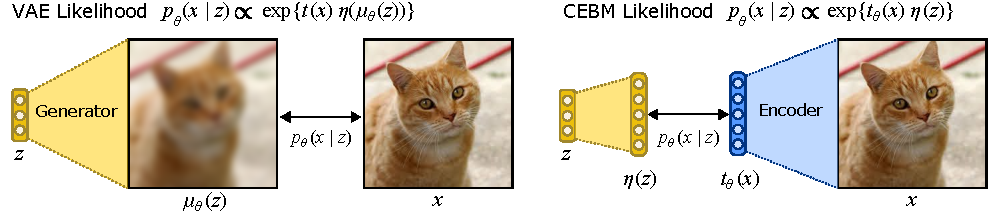
\includegraphics[width=\textwidth]{figures/cebm_overview_v2.pdf}
\vspace*{-4ex}
\caption{Comparison between the generative model in a VAE and CEBM. (\emph{Left}) In a VAE, the generator reconstructs an image $x$ by mapping the corresponding latent variable $z$ to pixel space to get a reconstruction $\mu_\q(z)$. The likelihood $p_\theta(x | z)$, defined by sufficient statistics $t(\cdot)$ and natural parameter $\eta(\cdot)$, can be interpreted as measuring the agreement between the image $x$ and its reconstruction $\mu_\q(z)$ in pixel space. The posterior in VAE is intractable and is approximated by an encoder network $q_\f(z|x)$. (\emph{Right}) A CEBM defines an energy-based likelihood that is defined by the neural sufficient statistics $t_\theta(\cdot)$ which serves as an encoder that maps $x$ to an intermediate-level representation, and the natural parameters $\eta(\cdot)$ that maps the latent variable $z$ to the same level. The likelihood $p_\theta(x | z)$ in a CEBM can be interpreted as measuring the agreement between $x$ and $z$ at their intermediate level of representations. In contrast to a VAE, the posterior in CEBM is tractable and is determined by sufficient statistics $t_\q(x)$ and natural parameters $\lambda_{\text{prior}}$.}
\label{fig:overview}
\end{figure*}

%This is feasible in simulated domains, such as 3D-rendered scenes \cite{lin2020space}, and we are seeing steady progress in specific domains such as images of faces \cite{vahdat2020nvae}. However, learning a high-quality generator poses challenges in more complex natural domains, such as streetview images \cite{law2019take}. 

%This leads us to consider the following questions. How can we perform unsupervised representation learning without following the approach set forth by VAEs of faithfully trying to reconstruct the input? Could such an approach lead to learning more semantically meaningful representations?

%\begin{comment}
This leads us to consider the question whether it is possible to develop alternatives to VAE-based architectures that can be used for learning representations in a fully unsupervised manner, but have a likelihood model that does not try to learn a pixel-perfect reconstruction of the input. In other words, is it possible that likelihood models that do not measure the agreement between latent variables and data at pixel level can learn more abstract representations, in the sense that it becomes easier to discard factors of variation that give rise to variation in pixel space, but should be considered noise?
%\end{comment}


In this paper, we consider energy-based models (EBMs) with latent variables as an alternative to VAEs. EBMs define an unnormalized density in terms of an energy function; high energies correspond to lower probabilities. The energy function is defined as a discriminative network rather than a generative network. Since EBMs do not attempt to learn a pixel-perfect reconstruction of the data, we can hope to learn more flexible densities that represents factors of variation at varying levels of precision.

% ; the set of features that is needed to determine whether the background of an image is representative of the training data is likely smaller than the set of features that would fully encode all pixels in the background.

%%%%%%%%%%%%%%%%%%
% AABI version
%%%%%%
% In this paper, we consider energy-based models (EBMs) with latent variables as an alternative VAEs for learning representations in an unsupervised manner. The general idea of using EBMs for this purpose is by no means new; it has a long history in the context of restricted Boltzmann machines (RBMs) and related models \citep{smolensky1986information, welling2005exponential, hinton2006fast}. Our motivation with the present work is to design a class of energy-based models that retain the desirable features of VAEs while addressing what we see as one of their main weaknesses: We would like incorporate inductive biases, but model the data at an intermediate level of representation that does not necessarily encode all features of an image at the pixel level. 
%%%%%%%%%%%%%%%%%%

%Since the energy function maps data to probabilities, EBMs are fundamentally discriminative m 
%and produces a single value corresponding to the energy for that particular data. There are two main advantages from using EBMs over other generative models (in particular VAEs): (1) The generative model is more flexible given it is not explicitly defined. (2) There is only a single network to train. However, unlike VAEs, EBMs directly model the data; there is no notion of latent variable. This is ofcourse not necessarily a problem if our target application is image generation or density estimation. However, this can be problematic if our target application is to extract meaningful features from the data. Moreover, impose we may want to impose an inductive bias on the features we learn (e.g. disentangled representation).  

%To date, EBMs have primarily been used to learn densities over training data \cite{}, or more generally class-conditional densities when labels are available \cite{}. 
Concretely, we propose conjugate EBMs (CEBMs), a new family of energy-based models in which the energy function defines a neural exponential family. While the normalizer of this family is intractable, we can nonetheless compute the posterior in closed form when we pair the likelihood with an appropriate conjugate prior. As a result, the neural sufficient statistics in a CEBM fully determine both the marginal likelihood and the encoder (Figure~\ref{fig:overview}), hereby side-stepping the need for a generator.

%%%%%%%%%%%%%%%%%%
% AABI version
%%%%%%
% Concretely, we propose Conjugate EBMs (CEBMs), a class of models in which the energy function defines a neural exponential family. While the normalizer of this family is intractable, we can compute its posterior in closed form when we pair the likelihood with an appropriate conjugate bias term in the energy function. As a result, the neural sufficient statistics in a CEBM fully determine both the marginal likelihood and the encoder, hereby side-stepping the need for a generator.
%%%%%%%%%%%%%%%%%%

%likelihood is an exponential family with an intractable normalizer. When we pair this likelihood with a matching conjugate prior, this results in a model with a tractable posterior. This means that if we train a CEBM by maximizing the marginal likelihood, the energy function fully determines both the marginal likelihood over training data 
%In this paper, we propose conjugate EBMs (CEBMs): a new family of energy-based generative models that both have a flexible likelihood and allows for imposing an inductive bias on the latent space. Our proposed model defines a joint energy function on both the data and a latent variable. We show that how conjugacy can be exploited in order train the log marginal likelihood of the data by marginalising over the latent variable. 

% We consider CEBMs with three types of priors. The first is a standard spherical Gaussian, which is common in the context of VAEs. We additionally consider two priors that combine continuous and discrete features. [TODO fix description; it is not clear to me what we mean by \emph{``For the first  extension, we show that how we can with a mixture model on the latent space. Second, we propose a Conjugate EBM that explicitly predicts both a discrete variable (class) and a continuous variable (style).''}] 

In our experiments, we evaluate the representations learned by CEBM using class labels
as a proxy for the primary factors of variation in a dataset. We show that CEBMs learn a notion of similarity that aligns more closely with class labels in the sense that nearest neighbors in the latent space are more likely to belong to the same class. Moreover, we show that the representations learned by CEBMs (in an unsupervised manner) can achieve a competitive performance in classification and out-of-distribution detection tasks.
%Finally, we show that CEBMs yield improvements relative to VAE-based models in semi-supervised settings, where a limited number of labels are available during training of the model. 
%%%%%%%%%%%%%%%%%%
% AABI version
%%%%%%
% In our experiments, we evaluate the representations learned by CEBM using class labels as a proxy for the primary factors of variation in a dataset. We show that CEBMs learn a notion of similarity that aligns more closely with class labels in terms of the nearest neighbors in latent space (Figure 1). Moreover, we show that the representations learned by CEBMs (in an unsupervised manner) can achieve a competitive performance in classification and out-of-distribution detection tasks.
%%%%%%%%%%%%%%%%%%

%The rest of the paper is structured as follows: In %Section \ref{sec:background} we provide an overview of %EBMs as well discussing the conjugacy relationship. We %then describe how conjugacy can be exploited to design %EBMs with latent variables in Section \ref{sec:cebm}. In %Section \ref{sec:related-work}, we discuss the relevant %prior work. Finally in Section \ref{sec:experiments}, we %perform a series of experiments on a variety of datasets %to demonstrate how our approach can both be used for %generating samples as well as learning a more meaningful %latent space compared to VAEs. 



Overall, our contributions can be summarized as follows:
\begin{enumerate}[noitemsep,topsep=0pt,parsep=6pt,partopsep=0pt]
    \item We propose CEBMs, a new class of energy-based models for unsupervised representation learning. Unlike VAEs, CEBMs model data not at a pixel, but at an intermediate representation level. Moreover, their joint density factorizes into a tractable posterior and an energy-based marginal over data. This means that CEBMs can be trained using existing methods for EBMs while still having inference being tractable at test time. 
    % \item We investigate . Concretely, we train CEBMs with two different inductive biases in order to investigate the helpfulness of inductive biases in latent space.
    \item We provide a discussion over various inductive biases that can be employed in CEBMs. Concretely, we show that two of the most common inductive biases in deep generative models can be incorporated in CEBMs: a spherical Gaussian and a mixture of Gaussians. 
    \item We evaluate this new class of models by running experiments that test the extent to which CEBMs learn representations that agree with class labels (which are not used during training). We show that CEBMs learn a latent space in which neighbors are more likely to belong to the same class, which translates to increased performance in few-label downstream classification tasks, and that CEBMs also perform competitively in out-of-domain detection tasks.
\end{enumerate}





%\begin{enumerate}
%\item We quantitatively verify that CEBMs can learn a %semantically more meaningful representation that can be %used for downstream tasks. 
%\item We demonstrate that CEBMs can be used for %generative modelling tasks such as generating high %fidelity images and out-of-domain detection. 
%\item We show that CEBMs can be trained in a %semi-supervised manner and is able to achieve competitive %accuracy compared to semi-supervised VAEs. 
%\end{enumerate}


% Explain the motivation of repsnetaiojn leanring. Take mayve somehthing from the rebuttle as well. Also to do taks like diensaglment, learning class and joint, we need models that allows to have different causeusal structures. 
% Why other EBMs have not been xplicty userd for generative models
% What flexnbility gives you that others give you. 
% by defining an unnormalized probability density over the data space





%%%%%%%%%%%%%%%%%%%%%%%%%%%%%%%%%%%%%%%%%%%%%%%%%%%%%%%%%%%%%%%%%%%%%%%%%%%%%%%%%%%%%%%%%%%%%%%%%%%%%%%%%
% \vspace*{-1.0ex}
\section{Background}
\label{sec:background}
% \vspace*{-1.0ex}
%%%%%%%%%%%%%%%%%%%%%%%%%%%%%%%%%%%%%%%%%%%%%%%%%%%%%%%%%%%%%%%%%%%%%%%%%%%%%%%%%%%%%%%%%%%%%%%%%%%%%%%%%


\subsection{Energy-Based Models}
% \vspace*{-1.5ex}
An EBM~\citep{lecun2006tutorial} defines a Gibbs-Boltzmann distribution density for $x\in\mathbb{R}^D$ as
% An EBM~\cite{lecun2006tutorial} on a space of configuration $x\in\mathbb{R}^D$ is a probabilistic model that defines a Gibbs-Boltzmann distribution over the possible configurations as 
\begin{align*}
    p_\q(x) &= \frac{\exp \left\{- E_\q(x)\right\}}{Z_\q},
    &
    Z_\q &= \int \!dx \: \exp \{- E_\q(x)\}.
\end{align*}
The function $E_\q(x) : \mathbb{R}^D \xrightarrow[]{} \mathbb{R}$ is called the energy function which maps each configuration to a scalar value, the energy of the configuration. This type of model is widely used in statistical physics, for example in Ising models.
The distribution can only be evaluated up to an unknown constant of proportionality, since computing the normalizing constant $Z_\q$ (also known as the partition function), requires an intractable integral with respect to all possible inputs $x$.

Our goal is to learn a model $p_\q(x)$ that is close to the true data distribution $p_\text{data}(x)$. A common approach for achieving this objective is to minimize the Kullback-Leibler divergence between the data distribution and the model, which is equivalent to maximizing the expected log-likelihood
\begin{align}
\label{eq:obj-ebm}
\mathcal{L}(\q)
&= \mathbb{E}_{p_\text{data}(x)}[\log p_\q (x)]
,\\ \nonumber
&= \mathbb{E}_{p_\text{data}(x)}[-E_\q (x)] - \log Z_\q.
\end{align}
The key difficulty when performing maximum likelihood estimation is that computing the gradient of $\log Z_\q$ is intractable. A common strategy is to express this gradient as an expectation with respect to $p_\q(x)$,
\begin{align}
    \nabla \log Z_\q 
    &= 
    \mathbb{E}_{p_\q(x')}
    \left[
    -\nabla_\q E_\q(x')
    \right]
    ,
\end{align}
which means that the gradient of $\mathcal{L}(\q)$ has the form
\begin{align*}
%\label{eq:grad-ebm}
\nabla_\q \mathcal{L}(\q)
&=
- \mathbb{E}_{p_\text{data}(x)}[\nabla_\q E_\q (x)] + \mathbb{E}_{p_\q(x')}[\nabla_\q E_\q(x')]
.
\end{align*}
This corresponds to \emph{maximizing} the probability of samples $x \sim p_\text{data}(x)$ from the data distribution and \emph{minimizing} the probability of samples $x' \sim p_\q(x')$ from the learned model. 

Contrastive divergence methods \cite{hinton2002training} compute a Monte Carlo estimate of this gradient. Estimating this gradient however requires samples from the model $x' \sim p_\q(x')$, which in turn requires approximate inference since this density is intractable. A common method for generating samples from the recent EBMs is Stochastic 
Gradient Langevin Dynamics (SGLD)~\cite{welling2011bayesian}, which initializes a sample $x'_0 \sim p_0(x')$ and then performs a sequence of gradient updates with additional injected noise $\epsilon$
\begin{align}
\label{eq:sgld}
% &
% x'_0 \sim p_0(x')
% , \\
x'_{i+1} &= x'_i - \frac{\alpha}{2} \frac{\partial E_\q (x')}{\partial x'} + \epsilon
\,,&
\epsilon &\sim N(0, \alpha)
.
\end{align}
SGLD is motivated as a discretization of a stochastic differential equation whose stationary distribution is equal to the posterior.
It is correct in the limit $i \to \infty$ and $\alpha \to 0$, but in practice will have a bias. 
%Moreover, it is common to independently tune the step size $\alpha$ and the variance of $\epsilon$ to allow for faster training~\cite{grathwohl2019your}.

The initialization $x'_0$ is crucial because it determines the number of steps needed to converge to a high-quality sample. For this reason, EBMs are commonly trained \cite{nijkamp2019anatomy, du2019implicit, grathwohl2019your} using persistent contrastive divergence (PCD)~\cite{tieleman2008training}, which initializes some samples from a replay buffer $\mathcal{B}$ of previously generated samples.

\comment{

% \subsection{Variational Autoencoders}
% \vspace*{-1.5ex}
% %Stochastic variational inference methods approximate the %posterior $p_\q(z | x)$ by learning a variational %distribution $q_\f(z | x)$ from some tractable family. 
% Variational autoencoders are a widely used class of deep generative models \cite{kingma2013auto-encoding, rezende2014stochastic}. A VAE defines a joint distribution $p_\q(\x, \z)$ over data $\x$ and latent variables $\z$; it combines an unstructured prior (e.g.~a spherical Gaussian) with a likelihood that is parameterized by an expressive neural network, often referred to as a decoder. An inference model, also known as an encoder, approximates the posterior $p_\q(\z \mid \x)$ by mapping each data point $x$ onto latent variables $z$. These models are trained by maximizing the stochastic evidence lower bound (ELBO) defined as
% %\vspace{-1.2em}
% \begin{align}
%     \label{eq:elbo}
%     \mathcal{L} (\f, \q)
%     &
%     = 
%     \E_{p_\text{data}(\x) \: q_\f(\z \mid \x)}
%     \left[
%       \log \frac{p_\q(\x, \z)}{q_\f(\z \mid \x)}
%     \right] 
%     % \\
%     % &
%     % =
%     % \E_{p^\textsc{data}(\x)}
%     % \left[
%     %     \log p_\q(x)
%     %     - 
%     %     \text{KL}(q_\f(\z \mid \x) \,||\, p_\q(\z \mid \x))
%     % \right]
% \end{align}
% When the $q_\f(z|x)$ is reparameterizable, we can compute Monte Carlo estimates of the gradient of this objective using pathwise derivatives. Non-reparameterizable cases, such as models with discrete variables, require likelihood-ratio estimators~\cite{williams1992simple}.

% Despite their successes, VAEs have limitations. By maximizing the ELBO, we favor encoder-decoder pair that perfectly reconstruct their input, so there is nothing preventing the VAE from mapping similar inputs to similar encoding, even when they might be semantically different. Likewise, examples that might be very dissimilar in pixel space because of noise or benign transformations might end up with very different latent representations. 

}

\subsection{Conjugate Exponential Families}
% \vspace*{-1.5ex}
An exponential family is a set of distributions whose probability density function or probability mass function can be expressed in the following form
\begin{align}
\label{eq:exponential-family}
    p(x \mid \eta) 
    &= 
    h(x) \exp \big\{ 
        t(x)^\top \eta   
        - A(\eta) \big\}.
\end{align}
where $h(\cdot)$ is a base measure, $\eta$ is a vector of natural parameters , $t(\cdot)$ is a vector of sufficient statistics, and $A(\cdot)$ is a log normalizer.

If a likelihood belongs to an exponential family, then there exists a conjugate prior with the same form
\begin{align}
    p(\eta \mid \lambda) 
    &= 
    h_0(\eta) \exp \big\{ 
    t_0(\eta)^\top \lambda
    - A_0(\lambda) \big\}.
\end{align}   
This prior is conjugate to the likelihood in~\ref{eq:exponential-family} when its vector of sufficient statistics comprises the natural parameters and the log-normalizer of the likelihood,
\begin{align}
% \label{eq:sufficient-stats}
    t_0(\eta) &= \big[ \eta, - A(\eta) \big], 
    &
    \lambda &= \big[ \lambda_1, \lambda_2 \big].
\end{align}
The convenient property of conjugate exponential families is that both the marginal likelihood $p(x \mid \lambda)$ and the posterior $p(\eta \mid x, \lambda)$ are tractable. The reason is that the joint probability has the form
\begin{align*}
    p(x, \eta \mid \lambda) &= p(x \mid \eta) \: p(\eta \mid \lambda)\\
    & 
    =h(x)h_0(\eta)\exp \big\{ 
      \eta^\top \! \big(\lambda_1 \!+\! t(x)\big) \\
      &
      \quad - A(\eta) (\lambda_2 \!+\! 1) 
      -
      A_0(\lambda)
    \big\}.
\end{align*}
If we substitute $\tilde{\lambda}_1 = \lambda_1 + t(x)$ and $\tilde{\lambda}_2 = \lambda_2 + 1$, then we can equivalently factorize this joint as
\begin{align}
    \label{eq:cef-joint}
    \begin{split}
    p(x, \eta \mid \lambda) &= p(\eta \mid x, \lambda) \: p(x \mid \lambda) \\
    & = p(\eta \mid \tilde{\lambda}) \: h(x) \exp\big\{ A_0(\tilde{\lambda}) - A_0(\lambda) \big\}.
    \end{split}
\end{align}
This shows that the posterior is in the same exponential family as the prior, and that we can express the marginal likelihood using $h(\cdot)$ and $A_0(\cdot)$
\begin{align}
    \label{eq:cef-posterior-and-marginal}
    \begin{split}
    p(\eta \mid x, \lambda) &= p(\eta \mid \tilde{\lambda}),
    \\
    p(x \mid \lambda) &= h(x)\exp\big\{ A_0(\tilde{\lambda}) - A_0(\lambda) \big\}.
    \end{split}
\end{align}
While conjugate exponential families have desirable properties, the class of tractable exponential families is limited. This is because it is in general not possible to compute the log normalizer for an arbitrary base measure $h(x)$ and a vector of sufficient statistics $t(x)$, which requires solving an integral with respect to $x$,
\begin{align}
    A(\eta) = \log \int dx \: h(x) \exp \big\{ t(x)^\top \eta  \}.
\end{align}
Similarly, not every exponential family has a tractable conjugate prior, since we need to be able to solve the integral for the log normalizer 
\begin{align}
    A_0(\lambda) = \log \int d\eta \: h_0(\eta) \exp \big\{ \eta^\top\lambda_1 - A(\eta)\lambda_2 \big\}.
\end{align}


%
% JWM: WROTE THIS WHOLE BIT BUT GOT RID OF IT. I THINK IT CONFUSES MORE THAN IT HELPS 
%

% In deep generative models, we can define an exponential family likelihood $p_\q(x \mid \eta_\q(z))$ in terms of a generator network $\eta_\q(z)$ that maps latent variables $z$ to a vector of natural parameters. This is in fact normal practice, since VAEs generally use a Gaussian or a Bernoulli likelihood, which are both exponential family distributions. However the corresponding conjugate prior $p_\q(z \mid \lambda)$ is intractable. This prior would have sufficient statistics $t_0(z) = [\eta_\q(z), -A(\eta_\q(z))]$ that are defined in terms of the generator network, which means that we cannot compute its log normalizer
% \begin{align}
%     A_0(\lambda) = \log \int dz \: \exp \big\{ \lambda_1^\top \eta_\q(z) - \lambda_2 A(\eta_\q(z)) \big\}. 
% \end{align}


%%%%%%%%%%%%%%%%%%%%%%%%%%%%%%%%%%%%%%%%%%%%%%%%%%%%%%%%%%%%%%%%%%%%%%%%%%%%%%%%%%%%%%%%%%%%%%%%%%%%%%%%%
\section{Conjugate Energy-Based Models}
\label{sec:cebm}
% \vspace*{-2.0ex}
%%%%%%%%%%%%%%%%%%%%%%%%%%%%%%%%%%%%%%%%%%%%%%%%%%%%%%%%%%%%%%%%%%%%%%%%%%%%%%%%%%%%%%%%%%%%%%%%%%%%%%%%%
% In this Section, we show that we can design energy functions such that the latent variable can be marginalized over by relying on the conjugacy relationship. Given a data point $\vx$, let $T_{\q}(\vx)$ be a set of sufficient statistics for data $\vx$. 

%To learn structured representations of the data $x$, we will design an energy-based %model that incorporates a latent space of $z$. Instead of learning reconstruction of %$z$ at the level of pixel space, we learn a 'relaxed likelihood' that measures the %agreement between data and latent variables at an intermediate level of %representation. Here we consider an unnormalized density

 

% Because most work on deep generative models has focused on images, we will restrict ourselves to this data modality. 

%Our goal is to learn a model in which latent variables $z$ reflect high-level features of interest, rather than low-level features that we might consider nuisance variables. 
In this paper we are interested in learning a probabilistic model that defines a joint distribution $p_\q(x, z)$ over high-dimensional data $x \in \mathbb{R}^D$ and a lower-dimensional set of latent variables $z \in \mathbb{R}^K$. The intuition that guides our work is that we would like to measure agreement between latent variables and data at a high level of representation, rather than at the level of individual pixels, where it may be more difficult to distinguish informative features from noise. To this end, we will explore energy-based models as an alternative to VAEs. 

Concretely, we propose to consider models of the form
\begin{align}
    p_\q(x, z) &= \frac{1}{Z_\q}\: \exp \big\{ -E_\q(x,z)\big\},
\end{align}
where the energy function takes a form that is inspired by exponential family distributions
\begin{align}
    \label{eq:cebm-energy}
    E_\q(x,z) = -t_\q(x)^\top \eta(z) - b(z).
\end{align}
In this energy function, $t_\q: \mathbb{R}^D \to \mathbb{R}^H$ plays the role of an encoder, which maps data to a vector of sufficient statistics. The function $\eta: \mathbb{R}^K \to \mathbb{R}^H$ decodes latent variables to a vector of natural parameters in an intermediate space of dimension H. The function $b: \mathbb{R}^K \to \mathbb{R}$ serves as an inductive bias that plays a role analogous to the prior. With this formulation, the generative model in a VAE can be recovered as a special case  that with this formulation (see Appendix~\ref{app:sec:vae}).

%Our intuition is that controlling the dimension $H$ may allow us to define energy functions that reflect agreement at a higher or lower level of representation. 

% For example, we can recover the generative model in a VAE as a special case. In this setting, $\eta_\q(z)$ is the generator network that maps low-dimensional latent variables to a high-dimensional vector of natural parameters. The function $t(x)$ is a known mapping of data to the sufficient statistics of a Gaussian or Bernoulli likelihood,
% \begin{align}
%     E_\q(x, z) = -t(x)^\top \eta_\q(z) - b_\q(z),
% \end{align}
% The bias $b_\q(z)$ contains the terms in the log density $\log p_\q(x,z)$ that only depend on $z$. In a VAE there are two such terms. The first is the log prior $\log p_\q(z)$. The second is the log normalizer of $A(\eta_\q(z))$ for the likelihood, which can be computed in closed form because Gaussian and Bernoulli distributions are in the exponential family. Combining these terms yields an energy function for the bias, 
% \begin{align}
%     \label{eq:vae-bias}
%     b_\q(z) = \log p_\q(z) - A(\eta_\q(z)).
% \end{align}
% In the middle of the spectrum, we could define a form
% \begin{align}
%     E_\q(x, z) = -t_\q(x)^\top \eta_\q(z) - b_\q(z).
% \end{align}
% Here, statistics at an intermediate level of representation are computed using a discriminative encoder network $t_\q(x)$, and natural parameters at the same intermediate level of representation are computed using a generator network $\eta_\q(z)$. The bias $b_\q(z)$ could take the form of a neural energy function, the logarithm of a deep generative prior $\log p_\q(z)$, or a combination of the two.

%This class of energy functions is the most general, in the sense that it allows us to define notions of agreement at varying levels of intermediate representation. However, these models may also be the most difficult to train, since both conditionals and marginals in the model will be intractable.
%
% More generally, we can define the energy in terms of an encoder network $t_\theta(x)$ that maps high-dimensional data to a low-dimensional vector of sufficient statistics. 

We will consider a bias $b(z) = \log p(z \mid \lambda)$ in form of a tractable exponential family with sufficient statistics $\eta(z)$\footnote{We drop the base measure for the rest of paper to avoid clutter.}, 
\begin{align}
    b(z) = \eta(z)^\top \lambda - A(\lambda).
\end{align}
We can then express the energy function as
\begin{align}
    E_\q(x, z) = -\big(\lambda + t_\q(x) \big)^\top \eta(z) + A(\lambda).
\end{align}
This form of the energy function has a very convenient property: It corresponds to a model $p_\theta(x,z)$ in which the posterior $p_\theta(z \mid x)$ is tractable. To see this, we make a substitution $\tilde{\lambda} = \lambda + t_\q(x)$ analogous to the one in Equation~\ref{eq:cef-joint}, which allows us to express the energy $E_\q(x, z)$ as
\begin{align}
    -\big(\eta(z)^\top \tilde{\lambda}  - A(\tilde{\lambda}) \big) -\big(A(\tilde{\lambda}) - A(\lambda) \big).
\end{align}
We now see that we can factorize the corresponding density $p_\q(x,z)$ as
\begin{align}
    p_\q(x,z \mid \lambda) 
    &= 
    p_\q(x \mid \lambda) \: p_\q(z \mid x, \lambda),
\end{align}
which yields a posterior and marginal that are analogous the distributions in Equation~\ref{eq:cef-posterior-and-marginal}%\footnote{Here, we drop the base measure $h(x)$},
\begin{align}
    p_\q(z \mid x, \lambda) &= p(z \mid \lambda + t_\q(x)),\\
    p_\q(x \mid \lambda) &= \frac{1}{Z_\q} \exp\big\{ A\big(\lambda + t_\q(x) \big) - A\big(\lambda\big) \big\}.
    \label{eq:cebm-marginal}
\end{align}
In other words, the joint density of this model factorizes into a tractable posterior $p_\theta(z \mid x, \lambda)$ and an intractable energy-based marginal likelihood $p_\theta(x \mid \lambda)$. This posterior is conjugate, in the sense that it is in the same exponential family as the bias. For this reason, we refer to this class of models as conjugate energy-based models (CEBMs).

CEBMs differ from VAEs in that they lack a generator network. Instead, the density is fully specified by the encoder network $t_\theta(x)$, which defines a notion of agreement $(\lambda + t_\q(x))^\top \eta(z)$ between data and latent variables in an intermediate feature space (see Figure~\ref{fig:overview}). In addition to having a tractable posterior, CEBMs have the convenient property that the marginal likelihood $p_\q(x \mid \lambda)$ itself can be expressed as an energy-based model that is defined in terms of the log normalizer $A(\cdot)$ and the encoder network $t_\q(x)$. This means that we can train CEBMs by maximizing the marginal likelihood $p_\q(x \mid \lambda)$ using PCD, in the same way that we would train other non-latent energy-based models \cite{du2019implicit,nijkamp2019anatomy}. 
% This procedure is described in Algorithm~\ref{alg:cebm}. 




% % \vspace*{-0.5ex}
\section{Inductive Biases}
% % \vspace*{-0.5ex}
CEBMs have a property that is somewhat counter-intuitive. While the posterior in $p_\q(z \mid x, \lambda)$ in this class of models is tractable, the prior $p_\q(z)$ is in general not tractable. In particular, although the bias $b(z)$ is the logarithm of a tractable exponential family, it is not the case that $p_\q(z) = \exp \{b(z)\}$. Rather the prior $p_\q(z)$ has the form,
\begin{align}
    p_\q(z) = \frac{\exp \{b(z)\}}{Z_\q} \ \int \! dx \: \exp \{t_\q(x)^\top \eta(z) \}.
\end{align}
In other words, the term $b(z)$ defines an inductive bias, but this bias is different from the bias in a VAE, where the prior is always tractable by construction\footnote{Concretely, the bias in a VAE (Eq.~\ref{eq:vae-bias}) contains the log prior $\log p_\q(z)$ and the log normalizer $A(\eta_\q(z))$ of the likelihood. In a CEBM, by contrast, we omit the second term $A_\q(\eta(z)) = \log \int dx \exp \{ t_\q(z)^\top \eta(z) \}$, which is intractable, and hereby implicitly incorporate it into the prior.}, but it imposes a soft constraint on the geometry of the latent space.


% \begin{figure}[!t]
% \centering
% 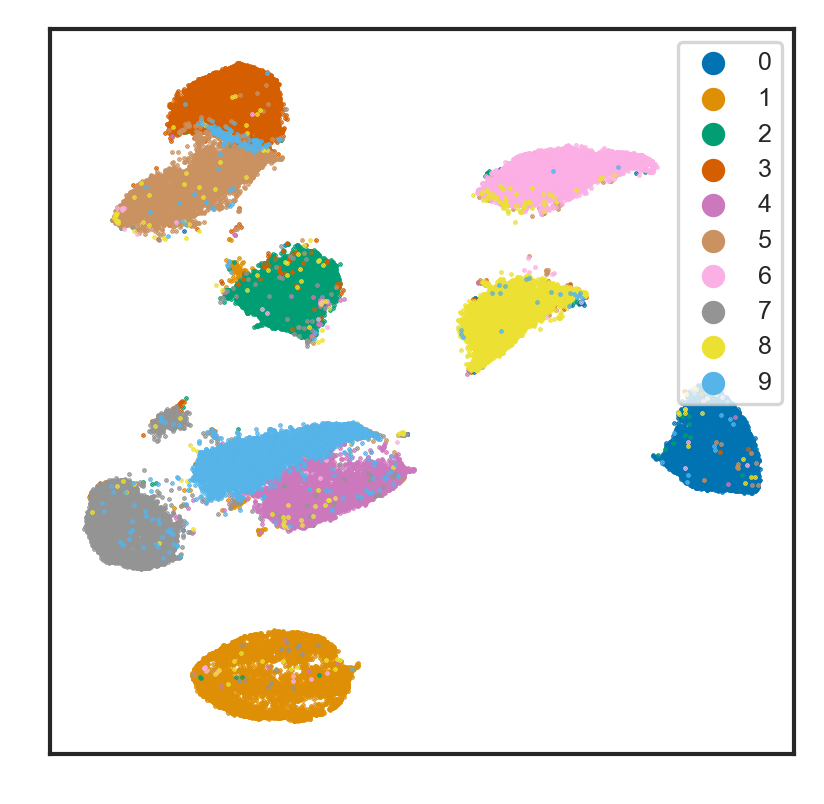
\includegraphics[width=0.48\linewidth]{figures/mnist_cebm_z_space.png}
% 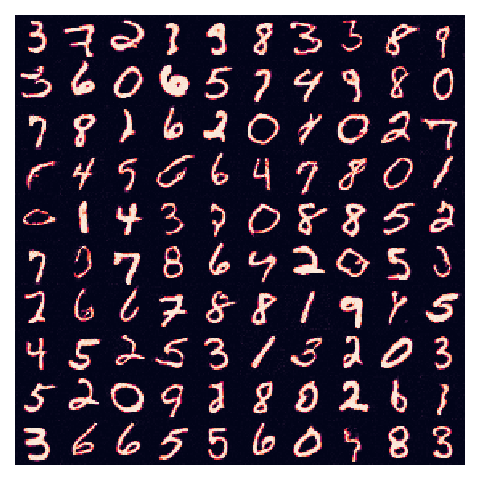
\includegraphics[width=0.48\linewidth]{figures/mnist_cebm_buffer_samples.pdf}
% \vspace*{-1.5ex}
% \caption{CEBM trained on MNIST; (\emph{Left}) latent space visualized with UMAP~\cite{mcinnes2018umap}. (\emph{Right}) Random samples generated from the model.}
% %\vspace*{-1.5ex}
% \label{fig:cebm-mnist}
% \end{figure}


%The bias in a VAE (Equation~\ref{eq:vae-bias}) differs from the bias in a CEBM in that it contains the log-normalizer of the likelihood in addition to the logarithm of the prior. In a CEBM we cannot compute this log-normalizer, since the integral with respect to $x$ will be intractable. For this reason, the term $b_\q(z)$ acts as an inductive bias, but this inductive bias does not constrain the learned representation in the same way as in a VAE, where the prior $p_\q(z)$ is tractable by construction. 

In principle the bias in a CEBM can take the form of any exponential family distribution. Since products of exponential families are also in the exponential family, this covers a broad range of possible biases. For purposes of evaluation in this paper, we will constrain ourselves to two cases:  

% for simplicity, eta in our case is not a neural network but a deterministic transformation between z and variables. 

\paragraph{1. Spherical Gaussian.} As a bias that is analogous to the standard prior in VAEs, we consider a spherical Gaussian with fixed hyperparameters $(\mu,\sigma)=(0,1)$ for each dimension of $z \in \mathbb{R}^K$,
\begin{align*}
    b(z) = \sum_{k} \big( \eta(z_k)^\top \lambda - A(\lambda) \big).
\end{align*}
Each term has sufficient statistics $\eta(z_k) = (z_k, z_k^2)$ and natural parameters
\begin{align*}
  \lambda = 
  \left(
      \frac{\mu}{\sigma^2},
      -\frac{1}{2\sigma^2}
  \right)
  =
  \left(
      0,
      -\frac{1}{2}
  \right)
  .
\end{align*}
The marginal likelihood of the CEBM is then
\begin{align*}
    p_\q(x \mid \lambda) 
    =
    \frac{1}{Z_\q}
    \exp \Big\{
      \sum_{k} \big(A(\tilde{\lambda}_k) - A(\lambda)\big)
    \Big\},
\end{align*}
where $\tilde{\lambda}_k = \lambda + t_{\q,k}(x)$ and the log normalizer is
\begin{align*}
    A(\tilde{\lambda}_k) 
    &=
    -\frac{\tilde{\lambda}_{k,1}^2}{4 \tilde{\lambda}_{k,2}}
    -
    \frac{1}{2} \log (-2\tilde{\lambda}_{k,2})
    .
\end{align*}

\paragraph{2. Mixture of Gaussians.} In our experiments, we will consider datasets that are normally used for classification. These datasets, by design, exhibit multimodal structure that we would like to see reflected in the learned representation. As an inductive bias that is amenable to uncovering this structure, we will consider a bias in the form of a mixture of $L$ Gaussians,
\begin{align*}
    b(y,z) = \sum_{k,l} I[y=l] \big( \eta(z_k)^\top \lambda_{l,k} - A(\lambda_{l,k}) \big).
\end{align*}
Here $z \in \mathbb{R}^K$ is a vector of features and $y \in \{1, \dots, L\}$ is a categorical assignment variable. The bias for each component $l$ is a spherical Gaussian with hyperparameters $\lambda_{l,k}$ for each dimension $k$. Again using the notation $\tilde{\lambda}_{l,k} = \lambda_{l,k} + t_{\q,l,k}(x)$ to refer to the posterior parameters, then we obtain an energy
\begin{align*}
    E_\q(x,y,z) =
    -
    \sum_{k,l}
    I[y=l]
    \big(  
        \tilde{\lambda}_{l,k}^\top \: \eta(z_k) 
        - A(\lambda_{l,k})
    \big).
\end{align*}
We can then define a joint probability over data $x$ and the assignment $y$ in terms the log normalizer $A(\cdot)$,
\begin{align*}
  & p_\q(x,y \,|\, \lambda) = \\
  & \qquad  
  \frac{1}{Z_\q(\lambda)}
  \exp \Big\{ 
    \sum_{k,l} 
    I[y=l]
    \big(
    A(\tilde{\lambda}_{l,k})
    -
    A(\lambda_{l,k})
    \big)
  \Big\},
\end{align*}
which then allows us to compute the marginal 
\begin{align*}
    p_\q(x \mid \lambda) = \sum_{y} p_\q(x,y \mid \lambda).
\end{align*}
We optimize this marginal with respect hyperaparameters $\lambda$ as well as the weights $\q$.


% So far we have shown that we can impose a Gaussian inductive bias on the latent space of CEBMs. However, one can argue that such inductive bias is too simple for most real-world datasets. Here, we ask the following question: can we impose a more structured inductive bias (e.g. a mixture model) on the latent space? It turns out that the answer is yes. Below, we will describe how to design such energy functions where the inductive bias on $z$ is a mixture model while we still are able to marginalize over it. 
% % We show that we can use the same conjugacy trick to design CEBMs where $\gamma_{\q}(x)$ can be computed analytically while the inductive bias on the latent space is a Gaussian mixture model.

% Let $y$ and $K$ be the cluster assignment, and the total number of clusters respectively. For simplicity, let's assume that every cluster has an equal probability of $\frac{1}{K}$. We now define the joint distribution over $z$ and $y$ as:
% \begin{equation}
% p(z, y \mid \lambda) = \frac{1}{K}\prod_{k=1}^{K}p(z \mid y=k,\lambda)^{I[y=k]}
% \end{equation}
% where $I$ is the identity function. We can re-write this distribution in an exponential form:
% \begin{equation}
% \label{eq:gmm-cebm-prior}
% \frac{1}{K} h(z) \exp \{\sum_{k=1}^K I[y=k]\left(\lambda^{T}_{k} t(z) - A_{0}(\lambda_{k})\right)\}
% \end{equation}
% where $\lambda_k$ is the natural parameters for the $k$'th mixture. The likelihood will have the same format as Eq.~\ref{eq:cebm-likelihood}. However, we can re-write the likelihood in a way to be conjugate to Eq.~\ref{eq:gmm-cebm-prior}:
% \begin{align}
% \gamma(x \mid z, y) 
% &= 
% \exp \{ \eta(z)^\top t_\q(x) \} \\
% &= \exp \{\sum_{k=1}^{K} I[y=k]\eta(z)^\top t_\q(x) \}
% \end{align}
% We now write the joint probability distribution over $x$, $z$, and $y$ as:
% \begin{align}
% \label{eq:cebmm-joint}
% p_{\q}(x,y,z)
% &=
% \frac{\gamma_{\q}(x,y,z)}{Z}
% \\
% \gamma_{\q}(x,y,z)
% &=
% \gamma_{\q}(x|y,z)p(z,y) 
% \end{align}
% This yield posterior distribution $p_{\q}(z|x,y)$ as:
% \begin{align}
% h(z)\exp \big\{\sum_{k=1}^{K} I[y=k]\left((\lambda_{k} + t_{\q}(x))^\top t(z) - A_{0}(\lambda_{k} + t_{\q}(x))\right) \big\}.  
% \end{align}
% and $\gamma_{\q}(x,z)$ as:
% \begin{align}
% \frac{1}{K}\exp \big\{ \sum_{k=1}^{K} I[y=k] \left(A_{0}(\lambda_k + t_{\q}(x)) 
%  - A_{0}(\lambda_k) \right) \big\}
% \end{align}
% By marginalizing over $y$, we can define $E_{\q}^{\textsc{CEBMM}}(x)$ as:
% \begin{equation}
% E_{\q}(x) = \frac{1}{K} \sum_{k=1}^{K} \exp \{A_{0}(\lambda_k + t_{\q}(x)) -  A_{0}(\lambda_k) \}
% \end{equation}

% %%%%%%%%%%%%%%%%%%%%%%%%%%%%%%%%%%%%%%%%%%%%%%%%%%%%%%%%%%%%%%%%%%%%%%%%%%%%%%%%%%%%%%%%%%%%%%%%%%%%%%%%%

% \vspace*{-0.5ex}
\section{Related Work}
\label{sec:related-work}
% \vspace*{-1.5ex}
%%%%%%%%%%%%%%%%%%%%%%%%%%%%%%%%%%%%%%%%%%%%%%%%%%%%%%%%%%%%%%%%%%%%%%%%%%%%%%%%%%%%%%%%%%%%%%%%%%%%%%%%%

% \comment{
% Energy-based models are popular in machine learning and can encompass a wide variety of models including basic classifiers, Markov Random Fields (MRF,~\cite{}), factor graphs, neural networks, exponential family, and Boltzmann machines. See~\cite{lecun2006tutorial} for a comprehensive tutorial on energy-based models. 

% In their general form, which can include latent variables, EBMs such as the ones we explore in this paper, as well as earlier models such as restricted Boltzmann machines (RBMs), are notoriously difficult to train.  Existing training methods employ Markov chain Monte Carlo (MCMC) sampling and include contrastive divergence (CD), its persistent variant (PCD) which is also known as stochastic maximum likelihood (SML), as well as rank-based methods \cite{hinton02training, tieleman2008training, younes1989parametric}.  Previous work examines and compares various ways of training EBMs \cite{swersky2011autoencoders}.

% Energy-based models \cite{lecun2006tutorial} have a long history in machine learning, in the sense that they admit many undirected models as special cases, including Markov random fields, factor graphs, and restricted Boltzmann machines (RBMs).
% }


% Our work focus on learning latent energy-based models in an unsupervised manner. 



% \begin{figure*}[!t]
% \centering
% 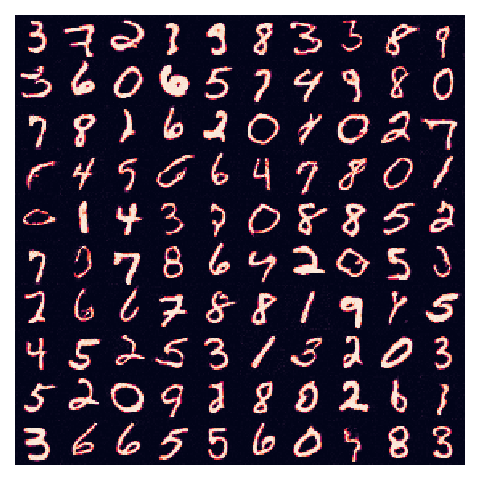
\includegraphics[width=0.235\textwidth]{figures/mnist_cebm_buffer_samples.pdf}
% 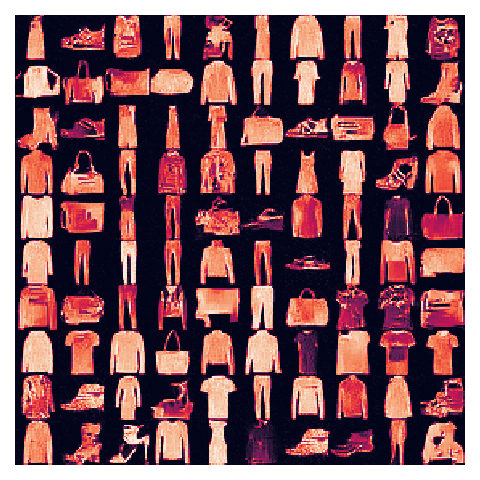
\includegraphics[width=0.235\textwidth]{figures/fmnist_cebm_samples.pdf}
% 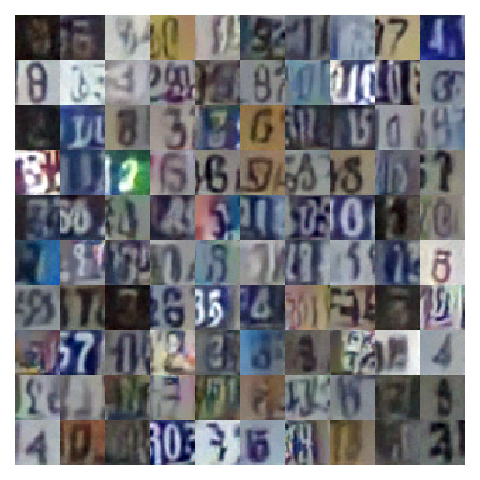
\includegraphics[width=0.235\textwidth]{figures/svhn_cebm_buffer_samples3.pdf}
% 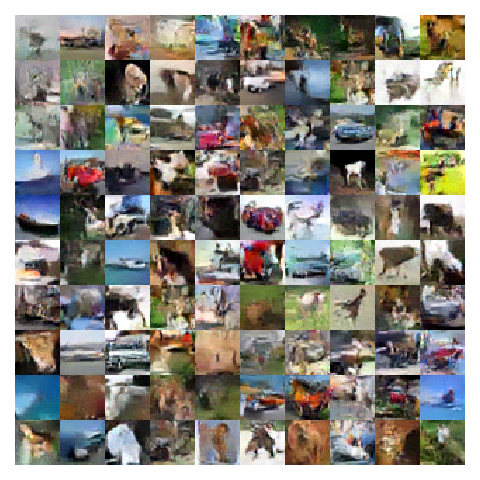
\includegraphics[width=0.235\textwidth]{figures/cifar10_cebm_buffer_samples.pdf}
% \vspace*{-1.5ex}
% \caption{Samples generated from a CEBM trained on MNIST, Fashion-MNIST, SVHN and CIFAR-10.}
% %\vspace*{-1.5ex}
% \label{fig:generated-samples}
% \end{figure*}




\paragraph{Energy-Based Latent Variable Models.} The general idea of using EBMs for representation learning is by no means new; it has a long history in the context of restricted Boltzmann machines (RBMs,~\citep{smolensky1986information,hinton2002training}), deep belief nets (DBNs,~\cite{hinton2006fast}), and deep Boltzmann machines (DBMs,~\citep{salakhutdinov2009deep}). The idea of extending RBMs in the exponential family and exploiting conjugacy to yield a tractable posterior is also not new and has been introduced in Exponential Family Harmonium~\citep{welling2005exponential}. Our motivation with the present work is to design a class of energy-based models that (1) are able to incorporate inductive biases in latent space, (2) model the data an intermediate level of representation using \emph{non-linear} transformations (unlike RBM-based models). The non-linearity of the relationship between the data and latent variables involves a trade-off; While it allows us to learn more complex distributions, it results in the likelihood no longer being tractable. We provide a more detailed discussion regarding the connection of our work to this class of models in Appendix~\ref{app:sec:rbm}.  


% \citet{welling2005exponential} propose a latent Harmonium model also in form of exponential family, where the joint density factorizes into a tractable posterior and a marginal. While this work shares with us the same property of tractable posterior, their model assumes one layer of hidden units with a bilinear energy function. 

% retain the desirable features of VAEs while addressing what we see as one of their main weaknesses: We would like incorporate inductive biases, but model the data at an intermediate level of representation that does not necessarily encode all features of an image at the pixel level. 

% EBMs~\cite{hinton2002training, lecun2006tutorial} is a broad class of probabilistic models in machine learning. Restricted Boltzmann Machines (RBMs,~\citet{hinton2012practical}), initially known as Harmoniums~\cite{smolensky1986information}, is one commonly used class of EBMs for representations learning. 



% \cite{nijkamp2019learning}. 


% \citet{gao2020flow} propose a flow-based EBM and interpret features from the top layer of the neural networks as latent representations.
% \paragraph{}

% Energy-based models \cite{lecun2006tutorial} have a long history in machine learning, in the sense that they admit many undirected models as special cases, including Markov random fields, factor graphs, and restricted Boltzmann machines (RBMs). Recent work on EBMs has shown that it is possible to use deep neural network as energy functions, and that it is possible to use Langevin methods to generate realistic samples from learned models \cite{du2019implicit,xie2016theory}. Work by \citet{grathwohl2019your} interprets classifiers through the lens of energy-based models. \citet{liu2020hybrid} propose a similar model where the objective combines a discriminative conditional and a generative conditional conditional distribution

% Recent work on EBMs has shown that it is possible to use deep neural network as energy functions, and that it is possible to use Langevin methods to generate realistic samples from learned models \cite{xie2016theory,nijkamp2019anatomy, nijkamp2019learning, du2019implicit}.

% Recent work has shown that EBMs with convolutional energy functions can accurately model distributions over images, in the sense that SGLD produces realistic samples \citep{nijkamp2019anatomy, nijkamp2019learning, du2019implicit,xie2016theory}. 

\paragraph{EBMs for Image Modelling.} Recent work has shown that EBMs with convolutional energy functions can accurately model distributions over images, yielding competitive results in image generation~\citep{xie2016theory,nijkamp2019anatomy,nijkamp2019learning, du2019implicit}. This line of work only focuses on generation and therefore do not consider incorporating latent variables in their models unlike our work. There has also been some work discussing the connection between EBMs and other successful deep learning models for images. For example, \citet{grathwohl2019your,liu2020hybrid} proposed to interpret a classifier as an EBM that defines a joint energy function on the data and labels. Similarly, \citet{che_your_2020} interprets a GAN as an EBM defined by both the generator and discriminator. Another line of work that is similar to ours in spirit is employing EBMs as priors on the latent space in deep generative models~\citep{pang2020learning,aneja2020ncp}. These models however, unlike our work, require a generator. \citet{nijkamp2019anatomy,nijkamp2019learning} performed a comprehensive analysis of convergence in recent EBMs, where they study a variety of factors such as MCMC chain initialization, network, and optimizer. They identify that a key factor for diagnosing these models is the difference between the energy of positive and negative samples. Many of these findings were helpful during the training and evaluation of EBMs in our work. 

% The same authors show that it is sometimes possible to learn a valid model even generate realistic samples even with a non-convergent, non-mixing short-run MCMC sampling 




% \citet{khemakhem2020ice} propose an EBM and a latent model in form of exponential family, for learning identifiable representations, i.e. for one dataset, the learned feature spaces by different encoders will be unique up to certain transformations. In contrast, we are interested in learning features that can represent meaningful factors of variations, which will be useful for a broad range of downstream tasks.  

% There has also been some work to address the instability problem in PCD~\citep{du2020improved}.

% Our motivation with the present work is to design a class of energy-based models that retain the desirable features of VAEs while addressing what we see as one of their main weaknesses: We would like incorporate inductive biases, but model the data at an intermediate level of representation that does not necessarily encode all features of an image at the pixel level. 

\paragraph{Training EBMs.} There is a large body of work on training unnormalized models. While our work as well as many others use PCD, we note that it is not the only approach for training EBMs. An alternative class of methods is Noise Contrastive Estimation (NCE)~\citep{gutmann2010noise} in which we define a noise model and learn by discriminating between data and noise. An example of this is \citet{gao2020flow}, where the authors pre-train a flow that acts as the noise model for training EBMs with NCE. Another popular approach is score matching (SM,~\citep{hyvarinen2005estimation,vincent2011connection,song2020sliced,bao_bi-level_2020}), in which we match the gradients of log probability density of the model and data distribution. Lastly, there are adversarial methods for avoiding MCMC sampling during MLE, where we introduce a variational distribution $q_{\f}(x)$ that we train alongside the model with a maximin objective~\citep{grathwohl2021no}. We refer the readers to~\citet{song2021train} for a more comprehensive study of training methods for EBMs. Note that because CEBMs can marginalize over $z$ to get the marginal, all of the discussed methods are available for training, and therefore are orthogonal to our work.   





 



% \paragraph{EBMs for Image Modelling.}  Recent work on EBMs has shown that it is possible to use deep neural network as energy functions, and that it is possible to use Langevin methods to generate realistic samples from learned models \cite{du2019implicit,xie2016theory}. Work by \citet{grathwohl2019your} interprets classifiers through the lens of energy-based models. \citet{liu2020hybrid} propose a similar model where the objective combines a discriminative conditional and a generative conditional conditional distribution. %\citet{yu2020training} show that EBMs can be trained not only with KL but with other f-divergences as well. 



% %%%%%Hao's Edit Starts%%%%%%%
% % talked about all ancient work before I was born...
% The first modern EBMs with energy functions as deep neural networks that were able to generate realistic samples with Langevin sampling were introduced by \citet{du2019implicit,xie2016theory}.
% \citet{nijkamp2019anatomy, nijkamp2019learning}
% %%%%%Hao's Edit Ends%%%%%%%%

%%%%%%%%%%%%%%%%%%%%%%%%%%%%%%%%%%%%%%%%%%%%%%%%%%%%%%%%%%%%%%%%%%%%%%%%%%%%%%%%%%%%%%%%%%%%%%%%%%%%%%%%%
\vspace*{-0.5ex}
\section{Experiments}
\label{sec:experiments}
% \vspace*{-1.5ex}
%%%%%%%%%%%%%%%%%%%%%%%%%%%%%%%%%%%%%%%%%%%%%%%%%%%%%%%%%%%%%%%%%%%%%%%%%%%%%%%%%%%%%%%%%%%%%%%%%%%%%%%%%


% \begin{figure}[!t]
% \centering
% 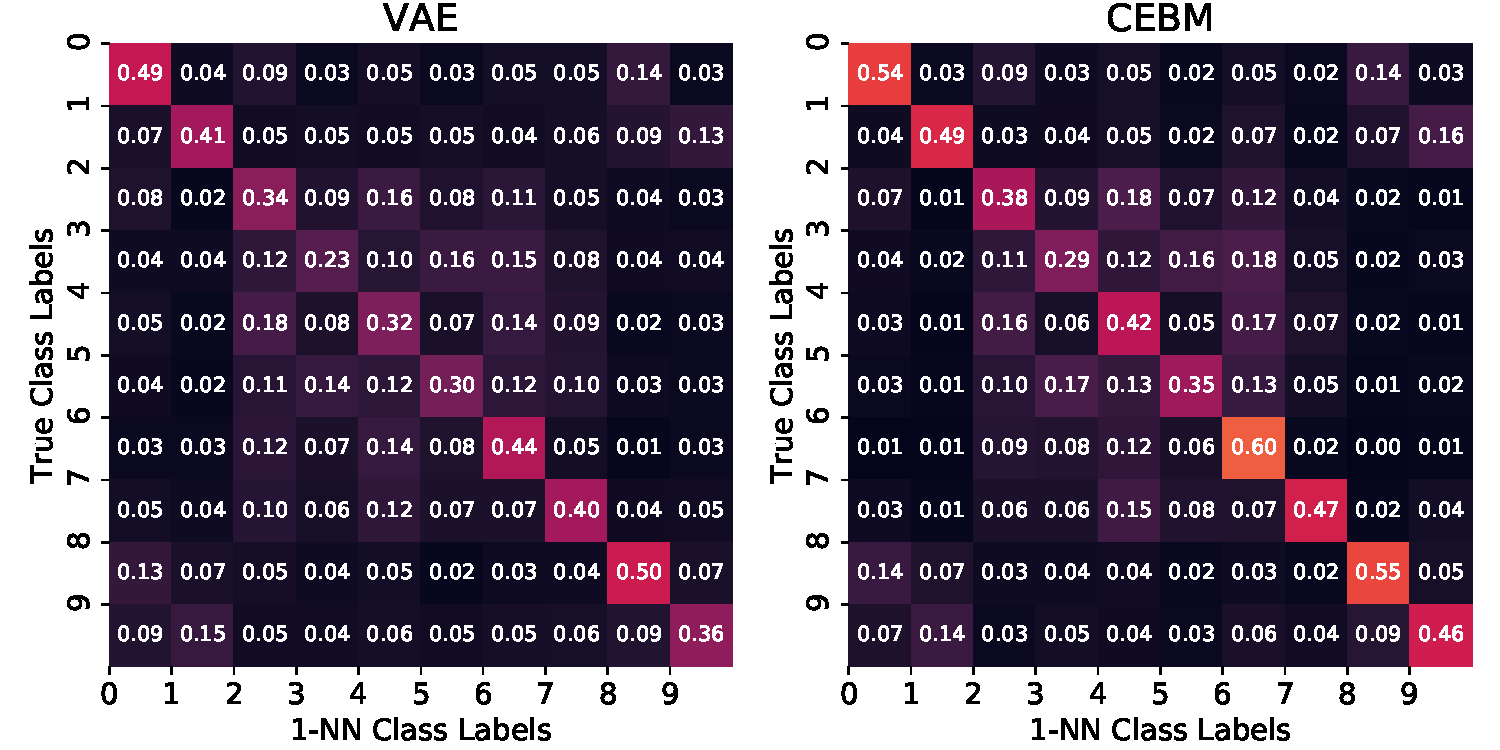
\includegraphics[width=\linewidth]{figures/confusion_matrix_22row_cifar10.pdf}
% \vspace*{-3.0ex}
% \caption{}
% \vspace*{-2.0ex}
% \label{fig:cebm-confusion-matrices}
% \end{figure}


\begin{figure}[!t]
\centering
\begin{subfigure}{0.22\textwidth}
\centering
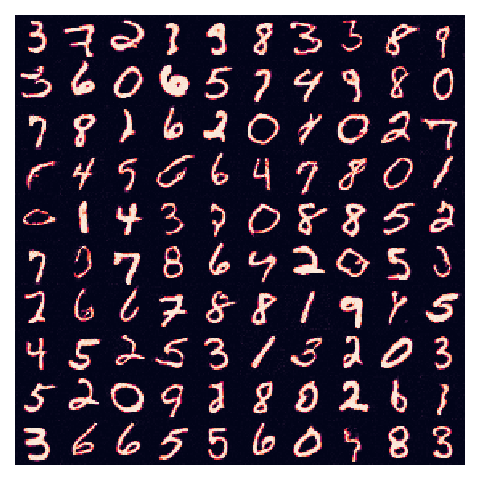
\includegraphics[width=\textwidth]{figures/mnist_cebm_buffer_samples.pdf}
\end{subfigure} %%
\begin{subfigure}{0.22\textwidth}
\centering
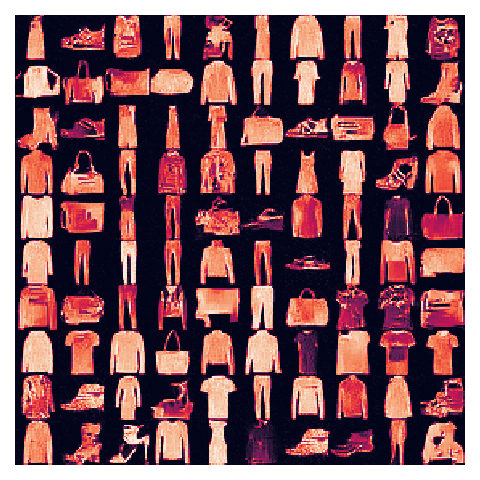
\includegraphics[width=\textwidth]{figures/fmnist_cebm_samples.pdf}
\end{subfigure}
\begin{subfigure}{0.22\textwidth}
\centering
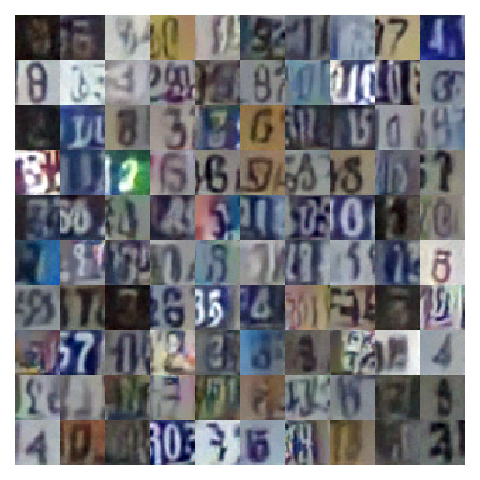
\includegraphics[width=\textwidth]{figures/svhn_cebm_buffer_samples3.pdf}
\end{subfigure} %%
\begin{subfigure}{0.22\textwidth}
\centering
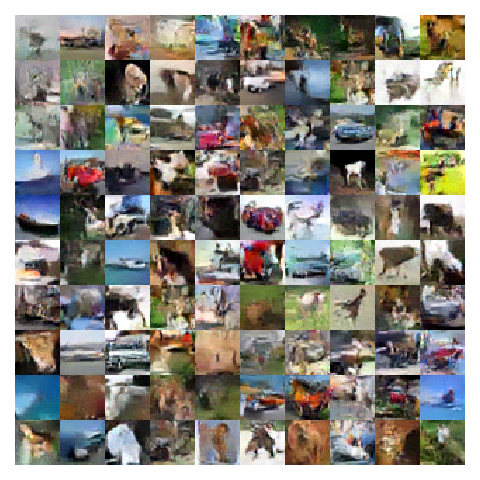
\includegraphics[width=\textwidth]{figures/cifar10_cebm_buffer_samples.pdf}
\end{subfigure}
% \vspace*{-1.5ex}
\caption{Samples generated from a CEBM trained on MNIST, Fashion-MNIST, SVHN and CIFAR-10.}
%\vspace*{-1.5ex}
\label{fig:generated-samples}
\end{figure}
Our experiments evaluate to what extent CEBMs can learn representations that encode meaningful factors of variation, whilst discarding details about the input that we would consider noise. This question is difficult to answer in generality, and in some sense not well-posed; whether a factor of variation should be considered signal or noise can depend on context. For this reason, our experiments primarily focus on the extent to which representations in CEBMs can recover the multimodal structure in datasets that are normally used for classification. %(MNIST~\cite{lecun1998gradient}, Fashion-MNIST~\cite{xiao2017fashion}, SVHN~\cite{netzer2011reading}, and CIFAR-10~\cite{krizhevsky2009learning}). 
While class labels are an imperfect proxy, in the sense that they do not reflect all factors of variation that we may want to encode in a representation, they provide a means of quantifying differences between representations that were learned in an unsupervised manner. 

We begin with a qualitative evaluation by visualizing samples and latent representation. We then demonstrate that learned representations align with class structure, in the sense that nearest neighbors in the latent space are more likely to belong to the same class (section~\ref{sec:exp:quality}). Next, we evaluate performance on out-of-distribution detection (OOD) tasks which, although not our primary focus in this paper, are a common use case for EBMs (Section~\ref{sec:exp:ood}).  %In the second experiment, we perform semi-supervised classification  (Section~\ref{sec:exp:semi}). 
Finally, to quantify the extent to which the learned representations can improve performance in downstream task, we measure low-label classification accuracy for representations that were pre-trained without supervision (Section~\ref{sec:exp:fewshots}).

%We design our experiments in an attempt to answer the following question: can CEBMs %learn a semantically more meaningful notion of representation compared to VAEs and %can this representation be used for downstream tasks such as classification? As a %proof of concept, we first visualize a few generated samples with SGLD to confirm %that we can successfully train CEBMs. Next, we examine the similarity between a few %random samples and their nearest neighbours in latent space. Lastly, we perform %classification on the latent code as an assessment of the quality of latent space. 






% \begin{table}[!b]
% \centering
% \begin{tabular}{lc}
% \toprule
%  &  FID \\
% \midrule
% GLOW  & 46.4 \\
% GMM-VAE   &  \\
% IGEBM & 37.9 \\
% CEBM  &   \\ 
% \bottomrule 
% \end{tabular}
% \caption{FID scores evaluated on CIFAR10.}
% \label{tab:fid-scores}
% \end{table}

% \begin{table}[!b]
% \centering
% \begin{tabular}{cccc}
% \toprule
% Glow & GMM-VAE   & IGEBM & CEBM \\
% \midrule
% 46.4  &           & 37.9  & \\
% \bottomrule
% \end{tabular}
% \caption{FID scores evaluated on CIFAR10}
% \label{tab:fid-scores}
% \end{table}


\vspace*{-1.ex}
\subsection{Network Architectures and Training}
\vspace*{-1ex}
% All CEBMs and EBMs in our experiments use an encoder network $t_\q(x)$ in the form of a 4-layer CNN. In the first layer we use kernel size 3 and stride 1. In subsequent layers we use kernel size 4 and stride 2~\cite{nijkamp2019anatomy}. The final layers are an MLP with 1024 and 512 hidden units, batch normalization, and Swish or LeakyReLU activation depending on the dataset. VAEs and GMM-VAEs use the same architecture for the encoder network, and use a decoder network that starts

\paragraph{Architectures.} CEBMs employ an encoder network $t_\q(x)$ in the form of 4-layer CNN (which is proposed by~\citet{nijkamp2019anatomy}), followed by an MLP output layer. For IGEBMs, we add one extra MLP as its final layer which outputs a scalar value. VAEs use the same encoder network as the CEBMs, and use a decoder network in form of an MLP followed by 4-layer CNN. See Appendix~\ref{appendix-architectures} for architecture details.

\paragraph{Optimization.} In CEBMs and VAEs we choose the dimension of latent variables to be 128. We found that the optimization becomes difficult with smaller dimensions. For training stability, we L2 regularize energy magnitudes (proposed by~\citet{du2019implicit}). We train our models using 60 SGLD steps, 90k gradient steps, batch size 128, Adam optimizer with learning rate 1e-4. See Appendix~\ref{app:sec:training-details} for training details.

\begin{figure}[!t]
\centering
\begin{subfigure}{0.42\textwidth}
\centering
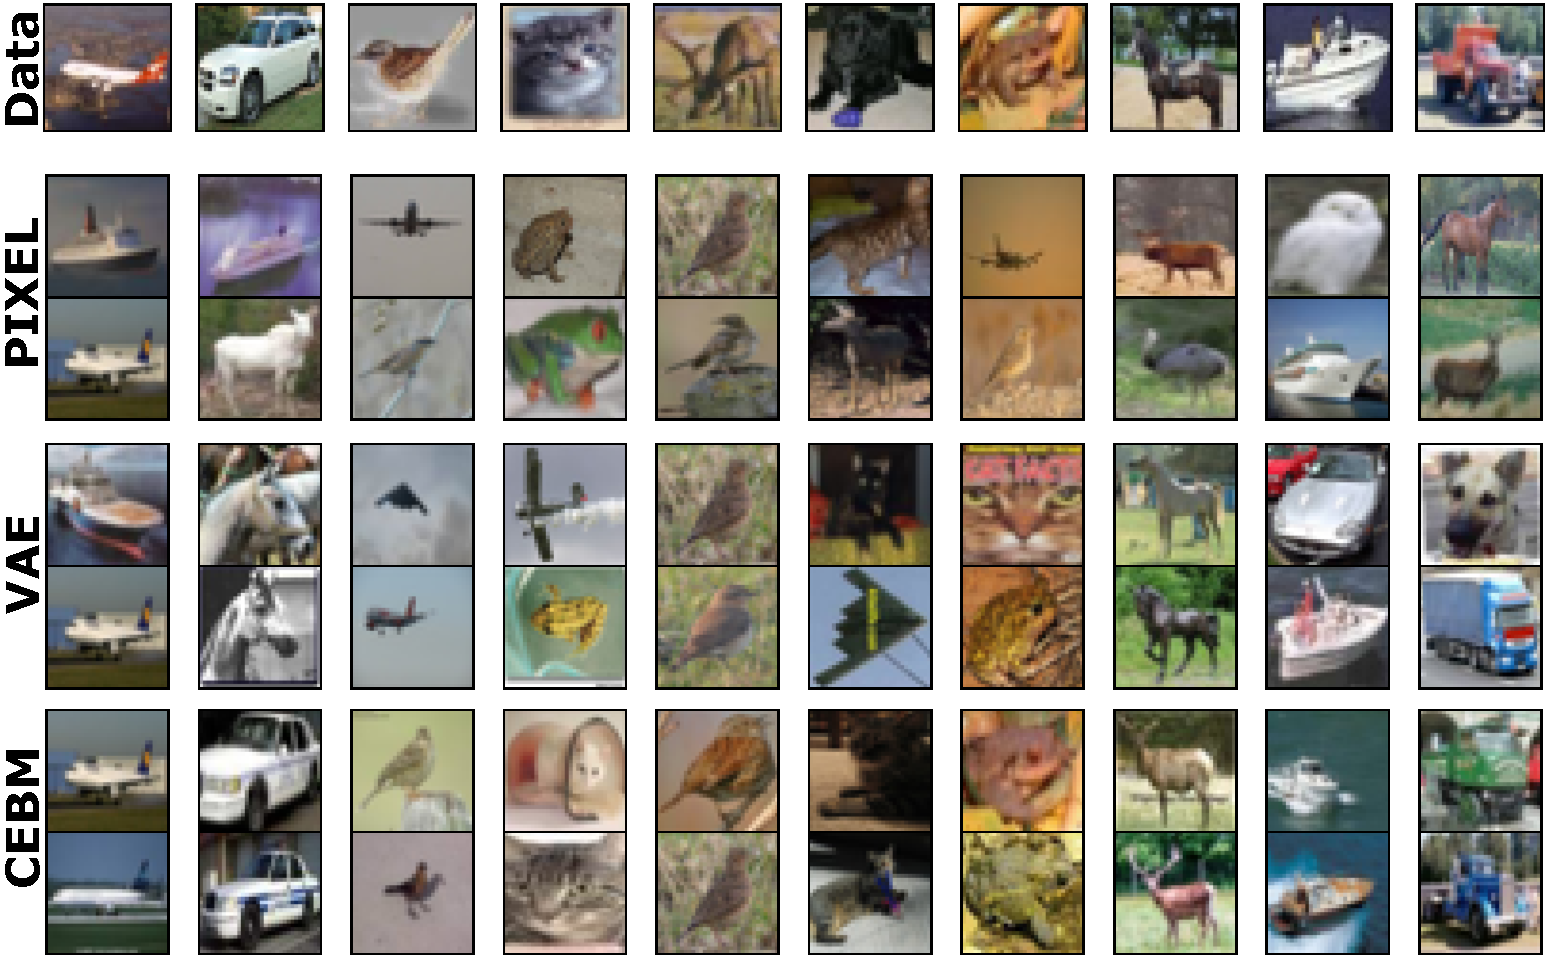
\includegraphics[width=\linewidth]{figures/overview_figure.pdf}
\end{subfigure}
\begin{subfigure}{0.45\textwidth}
\centering
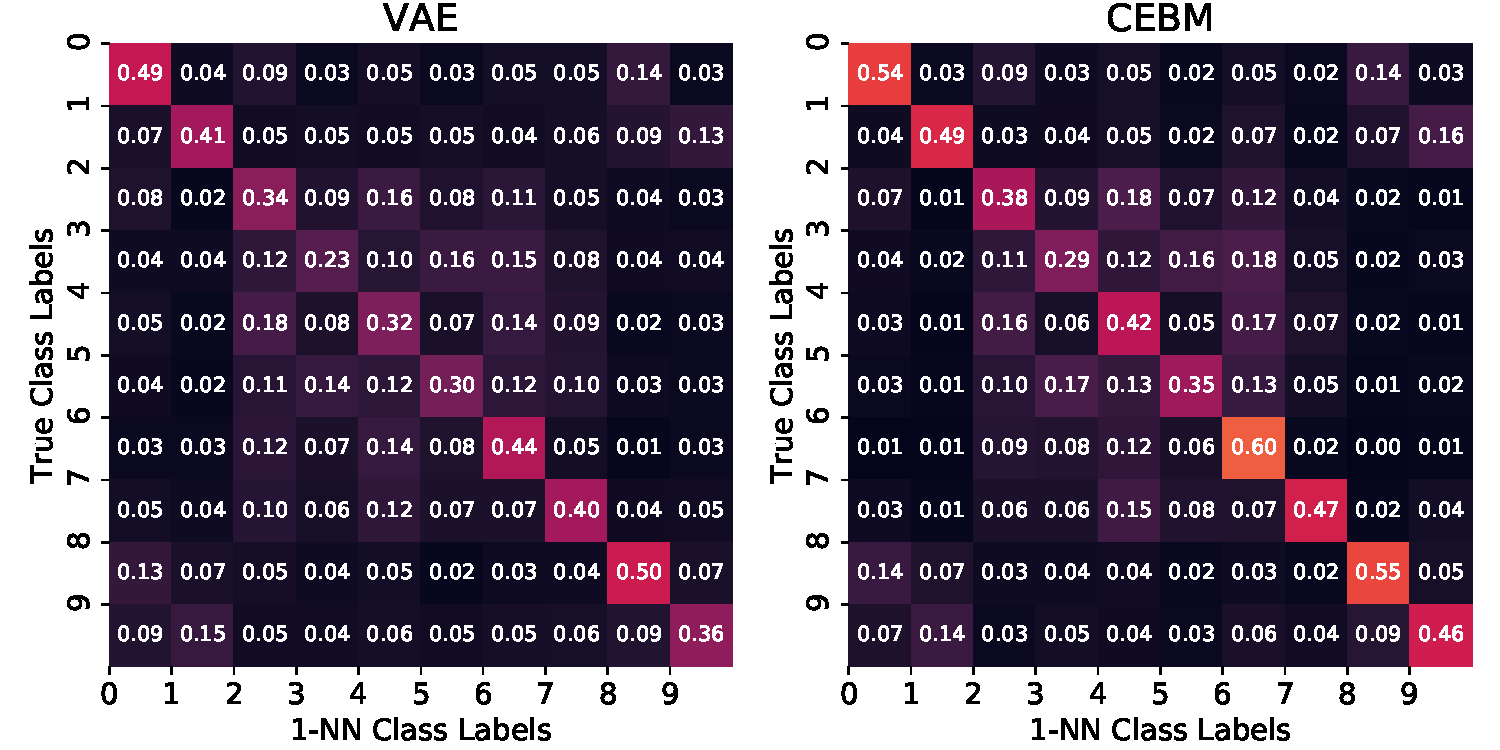
\includegraphics[width=\linewidth]{figures/confusion_matrix_22row_cifar10.pdf}
% \caption{Confusion Matrices of 1-nearest-neighbor classification on CIFAR10. We compute the L2 distance in the latent space to define neighbors of each testing example. The CEBM representation more closely aligns with class labels as compared to a VAE, as well as when compared to pixel-based and IGEBM-based baselines (additional results in Appendix~\ref{appendix-sec:confuion matrices}).}
\end{subfigure}
\caption{(\emph{Left}) Samples from CIFAR-10 along with the top 2-nearest-neighbors in pixel space, the latent space of a VAE, and the latent space of a CEBM. (\emph{Right}) Confusion matrices of 1-nearest-neighbor classification on CIFAR-10 based on L2 distance in the latent space. On average, CEBM representations more closely align with class labels compared to VAE.}
\label{fig:nearest-neighbours}
%\vspace*{-2.0ex}
\end{figure}

\begin{table*}[!t]
\caption{Classification accuracy. We pre-train 5 unsupervised models (rows) on MNIST, Fashion-MNIST, CIFAR10, SVHN. Then we train logistic classifiers using 1, 10, 100 examples per class (i.e. shots) and the full training dataset. We report the classification accuracy on the test set. We observe that CEBM outperforms the baselines in most scenarios.}
\centering
%\vspace*{-1.5ex}
\begin{tabular}{l|cccc|cccc|cccc|cccc}
\toprule
 & \multicolumn{4}{c}{MNIST} & \multicolumn{4}{|c}{Fashion-MNIST} & \multicolumn{4}{|c}{CIFAR-10} & \multicolumn{4}{|c}{SVHN}\\
Models & $1$ & $10$  & $100$ & $full$ & $1$ & $10$  & $100$ & $full$ & $1$ & $10$  & $100$ & $full$ & $1$ & $10$  & $100$ & $full$ \\
\midrule
\midrule
Classifier & 42 & 79 & 93 & 99 & 46 & 68 & 81 & 90 & 16 & 24 & 39 & 71 & 12 & 19 & 62 & 90\\
\midrule
VAE & 42 & 85 & 92 & 95 & 41 & 63 & 72 & 81 & 16 & 22 & 31 & 38 & 13 & 13 & 16 & 36\\
GMM-VAE & 53 & 86 & 93 & 97 & 49 & 68 & 79 & 84 & 19 & 23 & 33 & 39 & 13 & 14 & 23 & 56  \\
DCGAN & 9 & 13 & 13 & 14 & 10 & 11 & 16 & 17 & 10 & 11 & 12 & 13 & 9 & 11 & 12 & 20 \\
BIGAN & - & - & - & - & 51 & 70 & 76 & 81 & 17 & 26 & 36 & 45 & - & - & - & -  \\ 
\midrule
IGEBM & 63 & 89 & 95 & 97 & 50 & 70 & 79 & 83 & 16 & 26 & 33 & 42 & 10 & 16 & 35 & 49\\
CEBM & 67 & 89 & 95 & 97 & 52 & 70 & 77 & 83 & 19 & 30 & 42 & 52 & 12 & 25 & 48 & 70 \\
CEBMM & 67 & 91 & 97 & 98 & 52 & 71 & 80 & 85 & 16 & 28 & 42 & 51 & 10 & 17 & 39 & 60 \\
\bottomrule
\end{tabular}
\label{tab:few-shot classification}
\end{table*}

\paragraph{Hyperparameter Sensitivity.} As observed in previous work~\cite{du2019implicit,grathwohl2019your}, training EBMs can be a challenging task that often requires a thorough hyperparameter search. We found that the choices of activation function, learning rate, number of SGLD steps, and regularization will all affect training stability. Models regularly diverge during training, and it is difficult to perform diagnostics given that $\log p_{\q}(x)$ cannot be computed. As suggested by~\cite{nijkamp2019anatomy}, we found checking the difference in energy between data and model samples to be helpful for verifying stable training. We also note that in general, we observed a trade-off between sample quality and the predictive power of latent variables in our experiments. We leave investigation of the source of this trade-off to future work, but we suspect that this is because SGLD is having more difficulty to converge when the latent space is more disjoint.  



% \textbf{Models:}
% \begin{enumerate}
% \item $\gamma(\vx|\vz) = \text{exp}\left(\vz^{T}t_{\vtheta}(\vx) - (\vz^{2})^{T}t_{\vtheta}(\vx)^{2}\right)$
% \item $\gamma(\vx | \vz) = \text{exp}\left(\vz^{T}t_{\vtheta}(\vx) - (\vz^{2})^{T}t_{\vtheta}(\vx)^{2}\right) \\ p(\vz, \vy) = \frac{1}{K}\prod_{k}p(z|y=k)^{i[y==k]}$
% \item $\gamma(\vx| \vz, \vy) = \text{exp}\left(\vz^{T}t_{\vtheta}(\vx) - (\vz^{2})^{T}t_{\vtheta}(\vx)^{2}\right) \\ \text{exp}\left(f_{\q}(\vx)[y]\right)  \quad p(\vz, \vy) = p(\vz) p(\vy)$
% \item $\gamma(\vx| \vz, \vy) = \text{exp}\left(\vz^{T}t_{\vtheta}(\vx, \vy) - (\vz^{2})^{T}t_{\vtheta}(\vx, \vy)^{2}\right) \\ \text{exp}\left(f_{\q}(\vx)[y]\right)$
% \end{enumerate}


% \subsection{Latent Space Quality}

% In order to assess the quality of the latent space in CEBMs, we train a classifier on the training latent variables. Our results show that CEBMs can indeed learn a more meaningful latent space compared to VAEs.




% \begin{figure*}[!t]
% \centering
% \begin{subfigure}{0.4\textwidth}
% \centering
% 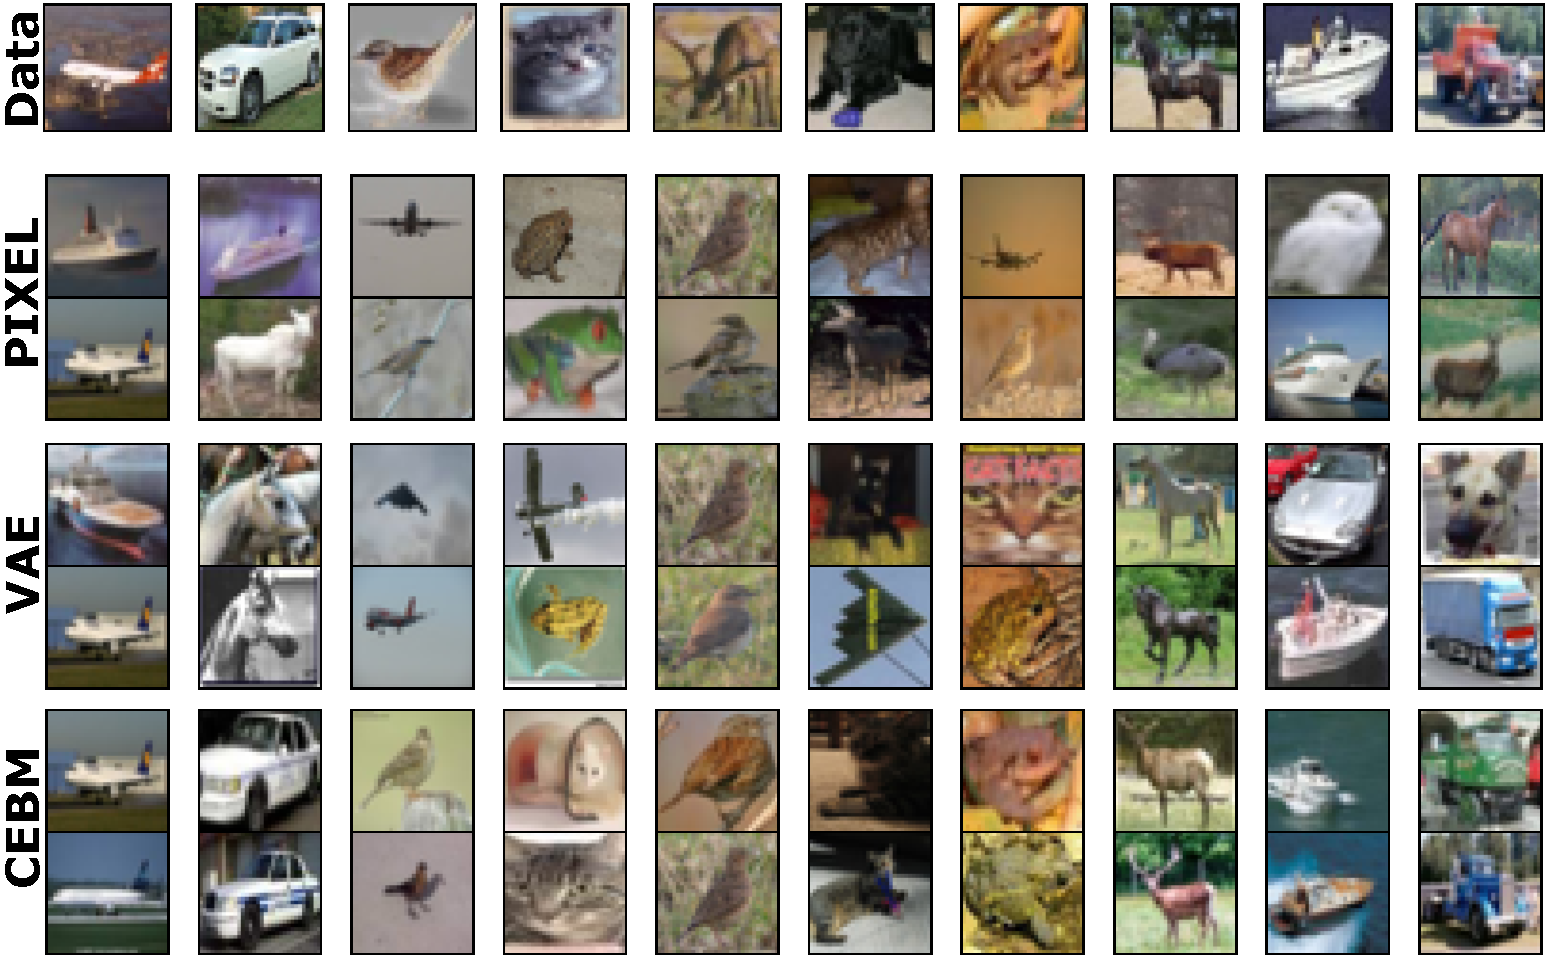
\includegraphics[width=\linewidth]{figures/overview_figure.pdf}
% \end{subfigure}%%%
% \begin{subfigure}{0.55\textwidth}
% \centering
% 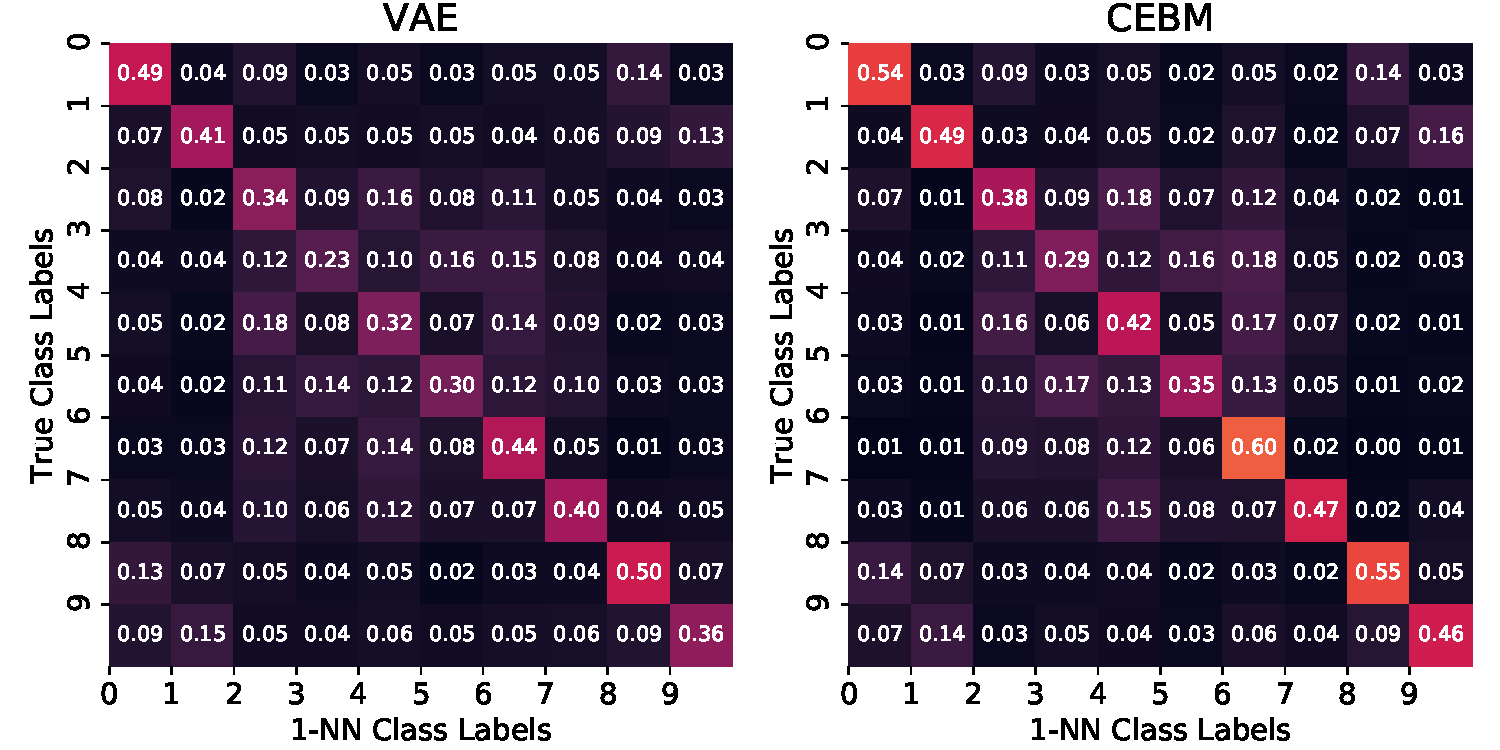
\includegraphics[width=\linewidth]{figures/confusion_matrix_22row_cifar10.pdf}
% % \caption{Confusion Matrices of 1-nearest-neighbor classification on CIFAR10. We compute the L2 distance in the latent space to define neighbors of each testing example. The CEBM representation more closely aligns with class labels as compared to a VAE, as well as when compared to pixel-based and IGEBM-based baselines (additional results in Appendix~\ref{appendix-sec:confuion matrices}).}
% \end{subfigure}
% \caption{(\emph{Left}) Samples from CIFAR-10 along with the top 2-nearest-neighbors in pixel space, the latent space of a VAE, and the latent space of a CEBM. (\emph{Right}) Confusion matrices of 1-nearest-neighbor classification on CIFAR-10 based on L2 distance in the latent space. On average, CEBM representations more closely align with class labels compared to VAE.}
% \label{fig:nearest-neighbours}
% %\vspace*{-2.0ex}
% \end{figure*}




\setlength{\tabcolsep}{4.5pt}
\begin{table*}[!t]
\caption{AUROC scores in OOD Detection. We use $\log p_{\q}(\x)$ and $\| \nabla_{\x}\log p_{\q}(\x)\|$ as score functions.The left block shows results of the models trained on F-MNIST and tested on MNIST, E-MNIST, Constant (C); The right block shows results of the models trained on CIFAR-10 and tested on SVHN, Texture and Constant (C).}
\centering
\begin{tabular}{l|ccc|ccc||ccc|ccc}
\toprule
& \multicolumn{6}{c||}{Fashion-MNIST} &    \multicolumn{6}{c}{CIFAR-10}\\
& \multicolumn{3}{c|}{$\log p_{\q}(\x)$} & \multicolumn{3}{c||}{$\| \nabla_{\x}\log p_{\q}(\x)\|$} &  \multicolumn{3}{c|}{$\log p_{\q}(\x)$} & \multicolumn{3}{c}{$\| \nabla_{\x}\log p_{\q}(\x)\|$}\\
\midrule
            &  MNIST  & E-MNIST& C &  MNIST & E-MNIST & C &  SVHN & Texture & C &  SVHN & Texture & C \\
\midrule
VAE         & .50 & .39 & .09 & .61 & .57 & .01  & .42 & \textbf{.58} & .41 & .38 & \textbf{.51} & .37 \\
IGEBM       & .35 & .36 & .90 & .78 & .82 & .96 & .45 & .31 & .64 & .33 & .17 & \textbf{.62} \\
CEBM        & .37 & .34 & .90 & \textbf{.82} & \textbf{.89} & \textbf{.98} & .47 & .32 & \textbf{.66} & .31 & .17 & .54 \\
CEBMM       & \textbf{.56} & \textbf{.56} & \textbf{.92} & .56 & .80 & .95     & \textbf{.55} & .30 & .62 & \textbf{.40} & .23 & \textbf{.62}  \\
\bottomrule
\end{tabular}
\label{tab:ood-detection}
\end{table*}


% \vspace*{-1.5ex}
\subsection{Samples and Latent Space}
\label{sec:exp:quality}
% \vspace*{-1.5ex}
% As with other EBMs~\cite{du2019implicit}, we can use SGLD to sample from CEBM. In Figures~\ref{fig:generated-samples} \&~\ref{fig:cebm-mnist}, we show generated samples from CEBM trained on different datasets by running 500 steps of SGLD. Even though the sample quality in CEBMs is far from state-of-the-art generative models, we observe that CEBMs do not suffer from blurriness as VAEs. Furthermore, these sample show that CEBMs are able to do a reasonable job at approximating the data distribution.

We begin with a qualitative evaluation by visualizing samples from the model. 
% Recent work has often focused on EBMs as an alternative to generative models~\cite{du2019implicit, nijkamp2019anatomy}, where it is natural evaluate model performance in terms of the the quality of generated samples. 
While generation is not our intended use case in this paper, such samples do serve as a useful diagnostic, in the sense that they allow us to visually inspect what characteristics of the input data are captured by the learned representation. 

Figures~\ref{fig:generated-samples} show samples from CEBMs trained on MNIST, Fashion-MNIST, SVHN, and CIFAR-10. We initialize the samples with uniform noise and run 500 SGLD steps. We observe that the distribution over images is diverse and captures the main characteristics of the dataset. Sample quality is roughly on par with samples from other EBMs \cite{nijkamp2019anatomy}, although it is possible to generate samples with higher visual quality using class-conditional EBMs~\cite{du2019implicit, grathwohl2019your, liu2020hybrid} (which assume access to labels).

% For a quantitative assessment, we report Frechet Inception Distance (FID)~\cite{heusel2017gans} where we compare against Glow~\cite{kingma2018glow}, GMM-VAE~\cite{tomczak2018vae}, and IGEBM~\cite{du2019implicit}. As shown in Table~\ref{tab:fid-scores}, CEBM is able to achieves a competitive FID score. 

To assess to what extent the representation in CEBMs aligns with classes in each dataset, we look at the agreement between the label for each data point and the label of its nearest neighbor in the latent space. In Figure~\ref{fig:nearest-neighbours}, we show samples from CIFAR-10, along with the images that correspond to the nearest neighbors in pixel space, the latent space of a VAE, and the latent space of a CEBM. The distance in pixel space is a poor measure of similarity in this dataset, whereas proximity in the latent space is more likely to agree with class labels in both VAEs and CEBMs. 

In Figure~\ref{fig:nearest-neighbours} (right), we quantify this agreement by computing the fraction of neighbors in each class conditioned on the class of the original image. We see a stronger alignment between classes and the latent representation in CEBMs, which is reflected in higher numbers on the diagonal of the matrix. On average, a fraction of 0.38 of the nearest neighbords are in the same class in the VAE, whereas 0.45 of the neighbors are in the same class in the CEBM. This suggest that the representation in CEBMs should lead to higher performance in downstream classification tasks. We will evaluate this performance in the next two experiments.

% \setlength{\tabcolsep}{5pt}
% \begin{table*}[!th]
% \caption{Classification accuracy. We pre-train 5 unsupervised models (rows) on MNIST, Fashion-MNIST, CIFAR10, SVHN. Then we train logistic classifiers using 1, 10, 100 examples per class (i.e. shots) and the full training dataset. We report the classification accuracy on the test set. We observe that CEBM outperforms the baselines in most scenarios.}
% \centering
% %\vspace*{-1.5ex}
% \begin{tabular}{l|cccc|cccc|cccc|cccc}
% \toprule
%  & \multicolumn{4}{c}{MNIST} & \multicolumn{4}{|c}{Fashion-MNIST} & \multicolumn{4}{|c}{CIFAR-10} & \multicolumn{4}{|c}{SVHN}\\
% Models & $1$ & $10$  & $100$ & $full$ & $1$ & $10$  & $100$ & $full$ & $1$ & $10$  & $100$ & $full$ & $1$ & $10$  & $100$ & $full$ \\
% \midrule
% \midrule
% Classifier & 42 & 79 & 93 & 99 & 46 & 68 & 81 & 90 & 16 & 24 & 39 & 71 & 12 & 19 & 62 & 90\\
% \midrule
% VAE & 42 & 85 & 92 & 95 & 41 & 63 & 72 & 81 & 16 & 22 & 31 & 38 & \textbf{13} & 13 & 16 & 36\\
% GMM-VAE & 53 & 86 & 93 & 97 & 49 & 68 & 79 & 84 & \textbf{19} & 23 & 33 & 39 & \textbf{13} & 14 & 23 & 56  \\
% \midrule
% GAN & -- & -- & -- & -- & -- & -- & -- & -- & -- & -- & -- & -- & -- & -- & -- & --\\
% GMM-GAN & -- & -- & -- & -- & -- & -- & -- & -- & -- & -- & -- & -- & -- & -- & -- & --  \\
% \midrule
% IGEBM & 63 & 89 & 95 & 97 & 50 & 70 & 79 & 83 & 16 & 26 & 33 & 42 & 10 & 16 & 35 & 49\\
% CEBM & \textbf{67} & 89 & 95 & 97 & \textbf{52} & 70 & 77 & 83 & \textbf{19} & \textbf{30} & \textbf{42} & \textbf{52} & 12 & \textbf{25} & \textbf{48} & \textbf{70}\\
% CEBMM & \textbf{67} & \textbf{91} & \textbf{97} & \textbf{98} &\textbf{52} & \textbf{71} & \textbf{80} & \textbf{85} & 16 & 28 & \textbf{42} & 51 & 10 & 17 & 39 & 60 \\
% \bottomrule
% \end{tabular}
% \label{tab:few-shot classification}
% \end{table*}


% \vspace*{-1.0ex}


% \vspace*{-1.0ex}
\subsection{Few-label classification}\label{sec:exp:fewshots}
% \vspace*{-1.0ex}

To evaluate performance in settings where few labels are available, we train a logistic classifier using $1, 10, 100$ examples per class, as well as the full training dataset. We compare CEBMs against the  IGEBM~\cite{du2019implicit}, a standard VAE  with the spherical Gaussian prior, and the GMM-VAE~\cite{tomczak2018vae} where the prior is a mixture of Gaussians. As discussed in Section~\ref{sec:background}, IGEBM does not have an explicit representation. In order to compare against IGEBM, we remove the last layer (which outputs the energy) and use the resulting intermediate representation as the latent code. 

We report the classification accuracy on the test set in Table~\ref{tab:few-shot classification}. We can see that that CEBMs overall achieve a higher accuracy compared to VAEs in particular for CIFAR-10 and SVHN where the pixel distance is not good measure for similarity. Moreover, we observe that CEBMs outperform IGEBM which suggest that the inductive biases in CEBMs can lead to increased performance in downstream tasks. 


\subsection{Out-of-Distribution Detection}\label{sec:exp:ood}
% \vspace*{-1.0ex}

EBMs have formed the basis for encouraging results in out-of-distribution (OOD) detection~\cite{du2019implicit,grathwohl2019your}. While it is not our focus in this paper, OOD detection can serve as an additional benchmark that helps evaluate whether a learned model accurately characterizes the data distribution. In Appendix~\ref{appendix-sec:ood-detection}, we report results in terms of two metrics. The first is the area under the receiver-operator curve (AUROC) when thresholding the log marginal $\log p_\q(x)$.  The second is the gradient-based score function proposed by ~\citet{grathwohl2019your}. CEBMs results for OOD detection in most cases improve upon VAE and IGEBM baselines.



% \begin{table*}[!h]
% \caption{OOD detection results. Models are trained on CIFAR-10 and tested on different OOD datasets: SVHN, Texture, and constant images. We use $\log p_{\q}(\vx)$ and $\| \nabla_{\vx}\log p_{\q}(\vx)\|$ as score functions..}
% \centering
% \begin{tabular}{l|ccc|ccc}
% \toprule
% & \multicolumn{3}{c|}{$\log p_{\q}(\vx)$} & \multicolumn{3}{c}{$\| \nabla_{\vx}\log p_{\q}(\vx)\|$} \\
% \midrule 
%             &  SVHN & Constant & Texture &  SVHN & Constant & Texture\\
% \midrule
% VAE         & 42 & 41 & \textbf{58} & 38 & 37 & \textbf{51} \\
% IGEBM       & 45 & 64 & 31 & 33 & \textbf{62} & 17 \\
% CEBM        & 47 & \textbf{66} & 32 & 31 & 54 & 17  \\
% CEBMM       & \textbf{55} & 62 & 30 & \textbf{40} & \textbf{62} & 23  \\
% \bottomrule
% \end{tabular}
% \label{tab:ood-detection}
% \end{table*}
% We employ CEBM as means of doing out-of-distribution (OOD) detection, where we do binary classification based on some score function as $s_\q (x) \in \mathbb{R}$.
% A good score function is upposed to assign high scores to in-distritbuion data and low scores to out-of-distribution data. A typical choice is to use the $s_\q(x) := \log p_\q(x)$, which means we fit a density model on the data and consider examples with low likelihood as OOD data. However, deep generative models like VAEs are not able to distinguish OOD data and will assgin higher likelihood to many OOD data points~\cite{nalisnick2018deep}. Based on this, we additionally use the gradient-based score funtion~\cite{grathwohl2019your}.

% We pre-trained different models on Fashion-MNIST and CIFAR-10, and perform OOD detection by different OOD datasets. To evaluate the performance, we compute the area under the receiver-operating curve (AUROC) score when classifying the in-distribution data and out-of-distribution data (see Table~\ref{tab:ood-detection}).


% \begin{table}[!t]
% \centering
% \begin{tabular}{ccc|ccc|ccc|ccc}
% \toprule
%      MNIST  & E-MNIST & Constant &  MNIST & E-MNIST & Constant &  SVHN & Constant & Texture &  SVHN & Constant & Texture\\
% \midrule
% 50 & 39 & 9 & 61 & 57 & 1 & 42 & 41 & \textbf{58} & 38 & 37 & \textbf{51} \\
% \bottomrule
% \end{tabular}
% \caption{AUROC scored computed for OOD Detection on various datasets for models trained on Fashion-MNIST and CIFAR-10.}
% \label{tab:ood-detection}
% \end{table}


% \begin{table*}[!h]
% \caption{AUROC; Out-of-Domain Detection.}
% \begin{subtable}[h]{\textwidth}
% \caption{OOD detection results. Models are trained on Fashion-MNIST and tested on different OOD datasets: MNIST, E-MNIST (digits subclass), and constant images. We use $\log p_{\q}(\vx)$ and $\| \nabla_{\vx}\log p_{\q}(\vx)\|$ as score functions.}
% \centering
% \begin{tabular}{l|ccc|ccc}
% \toprule
% & \multicolumn{3}{c|}{$\log p_{\q}(\vx)$} & \multicolumn{3}{c}{$\| \nabla_{\vx}\log p_{\q}(\vx)\|$} \\
% \midrule
%             &  MNIST  & E-MNIST & Constant &  MNIST & E-MNIST & Constant\\
% \midrule
% VAE         & 50 & 39 & 9 & 61 & 57 & 1 \\
% IGEBM       & 35 & 36 & 90 & 78 & 82 & 96 \\
% CEBM        & 37 & 34 & 90 & \textbf{82} & \textbf{89} & \textbf{98} \\
% CEBMM       & \textbf{56} & \textbf{56} & \textbf{92} & 56 & 80 & 95 \\
% \bottomrule
% \end{tabular}
% \vspace*{1ex}
% \end{subtable}
% \begin{subtable}[h]{\textwidth}
% \caption{OOD detection results. Models are trained on CIFAR-10 and tested on different OOD datasets: SVHN, Texture, and constant images. We use $\log p_{\q}(\vx)$ and $\| \nabla_{\vx}\log p_{\q}(\vx)\|$ as score functions..}
% \centering
% \begin{tabular}{l|ccc|ccc}
% \toprule
% & \multicolumn{3}{c|}{$\log p_{\q}(\vx)$} & \multicolumn{3}{c}{$\| \nabla_{\vx}\log p_{\q}(\vx)\|$} \\
% \midrule 
%             &  SVHN & Constant & Texture &  SVHN & Constant & Texture\\
% \midrule
% VAE         & 42 & 41 & \textbf{58} & 38 & 37 & \textbf{51} \\
% IGEBM       & 45 & 64 & 31 & 33 & \textbf{62} & 17 \\
% CEBM        & 47 & \textbf{66} & 32 & 31 & 54 & 17  \\
% CEBMM       & \textbf{55} & 62 & 30 & \textbf{40} & \textbf{62} & 23  \\
% \bottomrule
% \end{tabular}
% \end{subtable}
% \label{appendix-tab:ood-detection}
% \end{table*}


%%%%%%%%%%%%%%%%%%%%%%%%%%%%%%%%%%%%%%%%%%%%%%%%%%%%%%%%%%%%%%%%%%%%%%%%%%%%%%%%%%%%%%%%%%%%%%%%%%%%%%%%%
% \vspace*{-0.5ex}
\section{Conclusion}
\label{sec:conclusion}
% \vspace*{-0.5ex}
%%%%%%%%%%%%%%%%%%%%%%%%%%%%%%%%%%%%%%%%%%%%%%%%%%%%%%%%%%%%%%%%%%%%%%%%%%%%%%%%%%%%%%%%%%%%%%%%%%%%%%%%%

% aabi version
% We introduced CEBMs; a new family of energy-based models that define a joint energy function over both the data and latent variables. The joint distribution factorizes into a tractable posterior and a marginal likelihood, imposing an inductive bias on the latent space. This factorization allows us to directly optimize the marginal likelihood of the data, while at the same time imposing an inductive bias on the latent space. Experimental results for this class of models are encouraging; we observe a closer agreement between unsupervised representations and class labels, which translates into improvements in downstream classification tasks. 

% Unsupervised representation  is one of the key goals of training deep generative models. 
We introduced CEBMs; a new family of energy-based models that define a joint energy function over both the data and latent variables. The joint distribution in a CEBM factorizes into a tractable posterior and an intractable energy-based marginal likelihood. This factorization allows us to directly optimize the marginal likelihood of the data, while at the same time imposing an inductive bias on the latent space. Experimental results for this class of models are encouraging; we observe a closer agreement between unsupervised representations and class labels, which translates into improvements in downstream classification tasks relative to VAE-based baselines. This work opens up opportunities to explore conjugate energy-based models with structured bias terms as an alternative to models based on VAEs in settings where we are hoping to reason about structured representations with little or no supervision. 


% In the unusual situation where you want a paper to appear in the
% references without citing it in the main text, use \nocite
% \nocite{langley00}

\bibliography{references}
\bibliographystyle{icml2021}


%%%%%%%%%%%%%%%%%%%%%%%%%%%%%%%%%%%%%%%%%%%%%%%%%%%%%%%%%%%%%%%%%%%%%%%%%%%%%%%
%%%%%%%%%%%%%%%%%%%%%%%%%%%%%%%%%%%%%%%%%%%%%%%%%%%%%%%%%%%%%%%%%%%%%%%%%%%%%%%
% DELETE THIS PART. DO NOT PLACE CONTENT AFTER THE REFERENCES!
%%%%%%%%%%%%%%%%%%%%%%%%%%%%%%%%%%%%%%%%%%%%%%%%%%%%%%%%%%%%%%%%%%%%%%%%%%%%%%%
%%%%%%%%%%%%%%%%%%%%%%%%%%%%%%%%%%%%%%%%%%%%%%%%%%%%%%%%%%%%%%%%%%%%%%%%%%%%%%%
\appendix
% \documentclass{article}

% % Recommended, but optional, packages for figures and better typesetting:
% \usepackage{microtype}
% \usepackage{graphicx}
% % \usepackage{subfigure}
% \usepackage{booktabs} % for professional tables
% \usepackage{subcaption}
% \usepackage[noend]{algpseudocode}
% \usepackage{enumitem}
% \usepackage{amsmath}
% \usepackage{amssymb}

% % hyperref makes hyperlinks in the resulting PDF.
% % If your build breaks (sometimes temporarily if a hyperlink spans a page)
% % please comment out the following usepackage line and replace
% % \usepackage{icml2021} with \usepackage[nohyperref]{icml2021} above.
% \usepackage{hyperref}

% % Attempt to make hyperref and algorithmic work together better:
% \newcommand{\theHalgorithm}{\arabic{algorithm}}
% \usepackage{multirow}

% % Use the following line for the initial blind version submitted for review:
% \usepackage{icml2021}
% % operators

% \newcommand{\argmax}{\operatornamewithlimits{argmax}}
% \newcommand{\argmin}{\operatornamewithlimits{argmin}}

% vectors
\let\avec\vec
%\renewcommand{\vec}[1]{\ensuremath{\boldsymbol{#1}}}
\renewcommand{\v}[1]{\ensuremath{\boldsymbol{#1}}}

\newcommand{\src}{\lstinline[mathescape, keepspaces]}
\newcommand{\msrc}[1]{\mbox{\src!#1!}}

% \newcommand{\tens}[1]{%
%   \mathbin{\mathop{\otimes}\limits_{#1}}%
% }

% symbol shorthands (lowercase)
\newcommand{\x}{\ensuremath{\v{x}}}
\newcommand{\y}{\ensuremath{\v{y}}}
\newcommand{\z}{\ensuremath{\v{z}}}
\newcommand{\h}{\v{\eta}}
\newcommand{\e}{\v{\epsilon}}
\renewcommand{\u}{\v{u}}
\newcommand{\pd}{\ensuremath{\partial}}
% \newcommand{\x}{\ensuremath{x}}
% \newcommand{\y}{\ensuremath{y}}
% \newcommand{\z}{\ensuremath{z}}
% \newcommand{\h}{\ensuremath{\eta}}
% \newcommand{\e}{\ensuremath{\epsilon}}
\renewcommand{\u}{\ensuremath{u}}
\newcommand{\q}{\theta}
\newcommand{\f}{\phi}
\renewcommand{\l}{\lambda}
\renewcommand{\t}{\tau}

% symbol shorthands (uppercase)
\renewcommand{\L}{\ensuremath{\mathcal{L}}}
% \newcommand{\KL}[2]{\ensuremath{\mathrm{KL}\left({#1} \:\middle\vert\middle\vert\: {#2}\right)}}
\newcommand{\E}{\ensuremath{\mathbb{E}}}
\newcommand{\N}{\ensuremath{\mathcal{N}}}
\newcommand{\C}{\ensuremath{\mathtt{Concrete}}}

%\let\lmid\mid
%\renewcommand{\mid}{\!\lmid\!}

\newcommand{\eval}{\ensuremath{$\reflectbox{$\,\leadsto\,$}$}}
%\newcommand{\eval}{\sim}
\newcommand{\hide}[1]{}

\makeatletter
\DeclareRobustCommand{\cev}[1]{%
  \mathpalette\do@cev{#1}%
}
\newcommand{\do@cev}[2]{%
  \fix@cev{#1}{+}%
  \reflectbox{$\m@th#1\vec{\reflectbox{$\fix@cev{#1}{-}\m@th#1#2\fix@cev{#1}{+}$}}$}%
  \fix@cev{#1}{-}%
}
\newcommand{\fix@cev}[2]{%
  \ifx#1\displaystyle
    \mkern#23mu
  \else
    \ifx#1\textstyle
      \mkern#23mu
    \else
      \ifx#1\scriptstyle
        \mkern#22mu
      \else
        \mkern#22mu
      \fi
    \fi
  \fi
}

% % If accepted, instead use the following line for the camera-ready submission:
% %\usepackage[accepted]{icml2021}

% % The \icmltitle you define below is probably too long as a header.
% % Therefore, a short form for the running title is supplied here:
% \icmltitlerunning{Supplementary Materials}

% \begin{document}
\newpage
\onecolumn
\icmltitle{Supplementary Materials}
\appendix
\section{Model Architectures}
\label{appendix-architectures}
Table~\ref{appendex:tab:arch-cebm}, Table~\ref{appendex:tab:arch-vae}, and Table~\ref{appendex:tab:arch-igebm} show the architectures used for CEBM, VAE, and IGEBM, respectively.

\begin{table}[!h]
\caption{Architecture of CEBM}
    \centering
    \begin{subtable}[h]{.5\linewidth}
    \caption{MNIST and Fashion-MNIST.}
    \centering
        \begin{tabular}{|l|}
        \toprule
        \textbf{Encoder} \\
        \midrule
        Input $28\times28\times1$ images  \\
        \hline 
        $3\times3$ conv. 64 LeakyReLU. stride 1. padding 1  \\
        \hline 
        $4\times4$ conv. 64 LeakyReLU. stride 2. padding 1 \\
        \hline 
        $4\times4$ conv. 32 LeakyReLU. stride 2. padding 1  \\
        \hline
        $4\times4$ conv. 32 LeakyReLU. stride 2. padding 1 \\
        \hline
        FC. 128 LeakyReLU \\
        \hline
        FC. $2\times128$ \\
        \bottomrule
        \end{tabular}
    \end{subtable}%%%
    \begin{subtable}[h]{.5\textwidth}
    \caption{CIFAR10 and SVHN.}
    \centering
        \begin{tabular}{|l|}
        \toprule
        \textbf{Encoder}  \\
        \midrule
        Input $32\times32\times3$ images  \\
        \hline 
        $3\times3$ conv. 64 LeakyReLU. stride 1. padding 1  \\
        \hline 
        $4\times4$ conv. 128 LeakyReLU. stride 2. padding 1 \\
        \hline 
        $4\times4$ conv. 256 LeakyReLU. stride 2. padding 1  \\
        \hline
        $4\times4$ conv. 512 LeakyReLU. stride 2. padding 1  \\
        \hline
        FC. 128 LeakyReLU \\
        \hline
        FC. $2\times128$\\
        \bottomrule
        \end{tabular}
    \vspace*{1ex}
    \end{subtable}
    \label{appendex:tab:arch-cebm}
\end{table}



% \newpage
\begin{table}[!h]
\caption{Architecture of VAE}
    \centering
    \begin{subtable}[h]{\textwidth}
    \caption{MNIST and Fashion-MNIST.}
    \centering
        \begin{tabular}{|l|l|}
        \toprule
        \textbf{Encoder} & \textbf{Decoder} \\
        \midrule
        Input $28\times28\times1$ images & Input $z\in \mathbb{R}^{128}$ latent variables \\
        \hline 
        $3\times3$ conv. 64 LeakyReLU. stride 1. padding 1 & FC. 128 ReLU \\
        \hline 
        $4\times4$ conv. 64 LeakyReLU. stride 2. padding 1 & FC. $3\times3\times32$ ReLU \\
        \hline 
        $4\times4$ conv. 32 LeakyReLU. stride 2. padding 1 & $4\times4$ upconv. 32 LeakyReLU. stride 2. padding 1 \\
        \hline
        $4\times4$ conv. 32 LeakyReLU. stride 2. padding 1 & $4\times4$ upconv. 64 LeakyReLU. stride 2. padding 1 \\
        \hline
        FC. 128 ReLU & $4\times4$ upconv. 64 LeakyReLU. stride 2. padding 0 \\
        \hline
        FC. $2\times128$ & $3\times3$ upconv. 1 stride 1. padding 0 \\
        \bottomrule
        \end{tabular}
    \vspace*{1ex}
    \end{subtable}
    \begin{subtable}[h]{\textwidth}
    \caption{CIFAR10 and SVHN.}
    \centering
        \begin{tabular}{|l|l|}
        \toprule
        \textbf{Encoder} & \textbf{Decoder} \\
        \midrule
        Input $32\times32\times3$ images & Input $z\in \mathbb{R}^{128}$ latent variables \\
        \hline 
        $3\times3$ conv. 64 LeakyReLU. stride 1. padding 1 & FC. 128 ReLU \\
        \hline 
        $4\times4$ conv. 128 LeakyReLU. stride 2. padding 1 & FC. $4\times4\times512$ ReLU \\
        \hline 
        $4\times4$ conv. 256 LeakyReLU. stride 2. padding 1 & $4\times4$ upconv. 32 LeakyReLU. stride 2. padding 1 \\
        \hline
        $4\times4$ conv. 512 LeakyReLU. stride 2. padding 1 & $4\times4$ upconv. 64 LeakyReLU. stride 2. padding 1 \\
        \hline
        FC. 128 ReLU & $3\times3$ upconv. 64 LeakyReLU. stride 2. padding 1 \\
        \hline
        FC. $2\times128$ & $3\times3$ upconv. 1 stride 1. padding 1 \\
        \bottomrule
        \end{tabular}
    \vspace*{1ex}
    \end{subtable}
    \label{appendex:tab:arch-vae}
\end{table}

\begin{table}[!h]
\caption{Architecture of IGEBM}
    \centering
    \begin{subtable}[h]{.5\textwidth}
    \caption{MNIST and Fashion-MNIST.}
    \centering
        \begin{tabular}{|l|}
        \toprule
        \textbf{Encoder} \\
        \midrule
        Input $28\times28\times1$ images  \\
        \hline 
        $3\times3$ conv. 64 LeakyReLU. stride 1. padding 1  \\
        \hline 
        $4\times4$ conv. 64 LeakyReLU. stride 2. padding 1 \\
        \hline 
        $4\times4$ conv. 32 LeakyReLU. stride 2. padding 1  \\
        \hline
        $4\times4$ conv. 32 LeakyReLU. stride 2. padding 1 \\
        \hline
        FC. 128 LeakyReLU \\
        \hline
        FC. 128 LeakyReLU. FC. 1 \\
        \bottomrule
        \end{tabular}
    \end{subtable}%%%
    \begin{subtable}[h]{.5\textwidth}
    \caption{CIFAR10 and SVHN.}
    \centering
        \begin{tabular}{|l|}
        \toprule
        \textbf{Encoder}  \\
        \midrule
        Input $32\times32\times3$ images  \\
        \hline 
        $3\times3$ conv. 64 LeakyReLU. stride 1. padding 1  \\
        \hline 
        $4\times4$ conv. 128 LeakyReLU. stride 2. padding 1 \\
        \hline 
        $4\times4$ conv. 256 LeakyReLU. stride 2. padding 1  \\
        \hline
        $4\times4$ conv. 512 LeakyReLU. stride 2. padding 1  \\
        \hline
        FC. 128 LeakyReLU \\
        \hline
        FC. 128 LeakyReLU. FC. 1\\
        \bottomrule
        \end{tabular}
    \vspace*{1ex}
    \end{subtable}
    \label{appendex:tab:arch-igebm}
\end{table}

\section{Training Details}
\label{appendix-sec:training-details}
In CEBMs and VAEs, we choose the dimension of latent variables to be 128. For CEBMS, We found that the optimization becomes difficult with smaller dimensions. We L2 regularize energy magnitudes (proposed by~\citet{du2019implicit}), where the coefficient of the L2 regularization term is 0.1. We empirically found that the training would become unstable without this regularization. We train our models using 60 SGLD steps where we initialize samples from the replay buffer with 0.95 probability, and initialize from uniform noise with 0.05 probability. We train all the models with 90k gradient steps, batch size 128, Adam optimizer with learning rate 1e-4. When doing PCD, we used a reply buffer of size 5000. We set the $\alpha$ in the SGLD teps to be 0.075. Similar to~\citet{du2019implicit}, we found it useful to add some noise to the image before encoding. In our experiments, we used Gaussian noise with $\sigma^{2} = 0.03$. For the mixture models (CEBMM and GMM-VAE), we used 50 mixtures.  

\newpage
\section{Additional Results}
\label{app:sec:additional-results}

\subsection{Confusion Matrices on 1-NN Classification}
\label{appendix-sec:confuion matrices}
We perform 1-nearest-neighbor classification task for MNIST, Fashion-MNIST, SVHN, CIFAR10. We compute the L2 distance in the latent space of VAE, IGEBM and CEBM, and also in pixel space. We visualize the confusion matrices
\begin{figure}[!h]
\centering
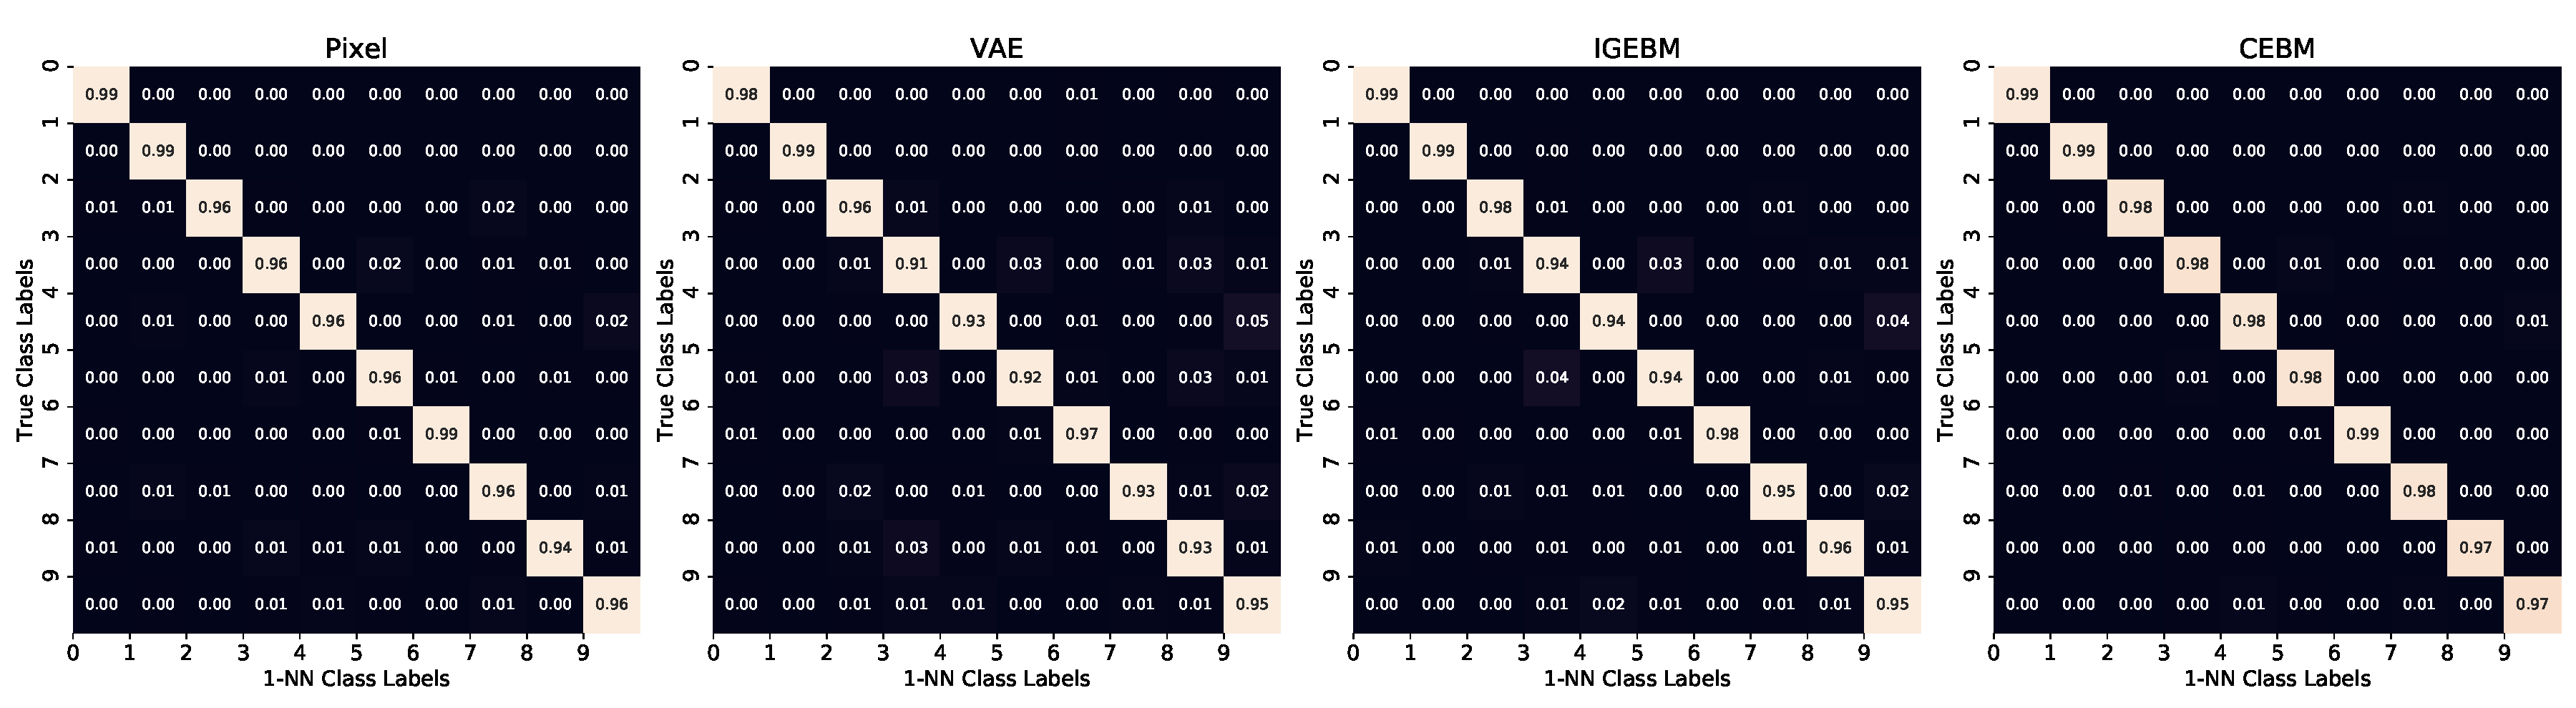
\includegraphics[width=\linewidth]{figures/confusion_matrix_14row_mnist.pdf}
\caption{MNIST}
\label{appendix:confusion-matrices-mnist}
\end{figure}
\begin{figure}[!h]
\centering
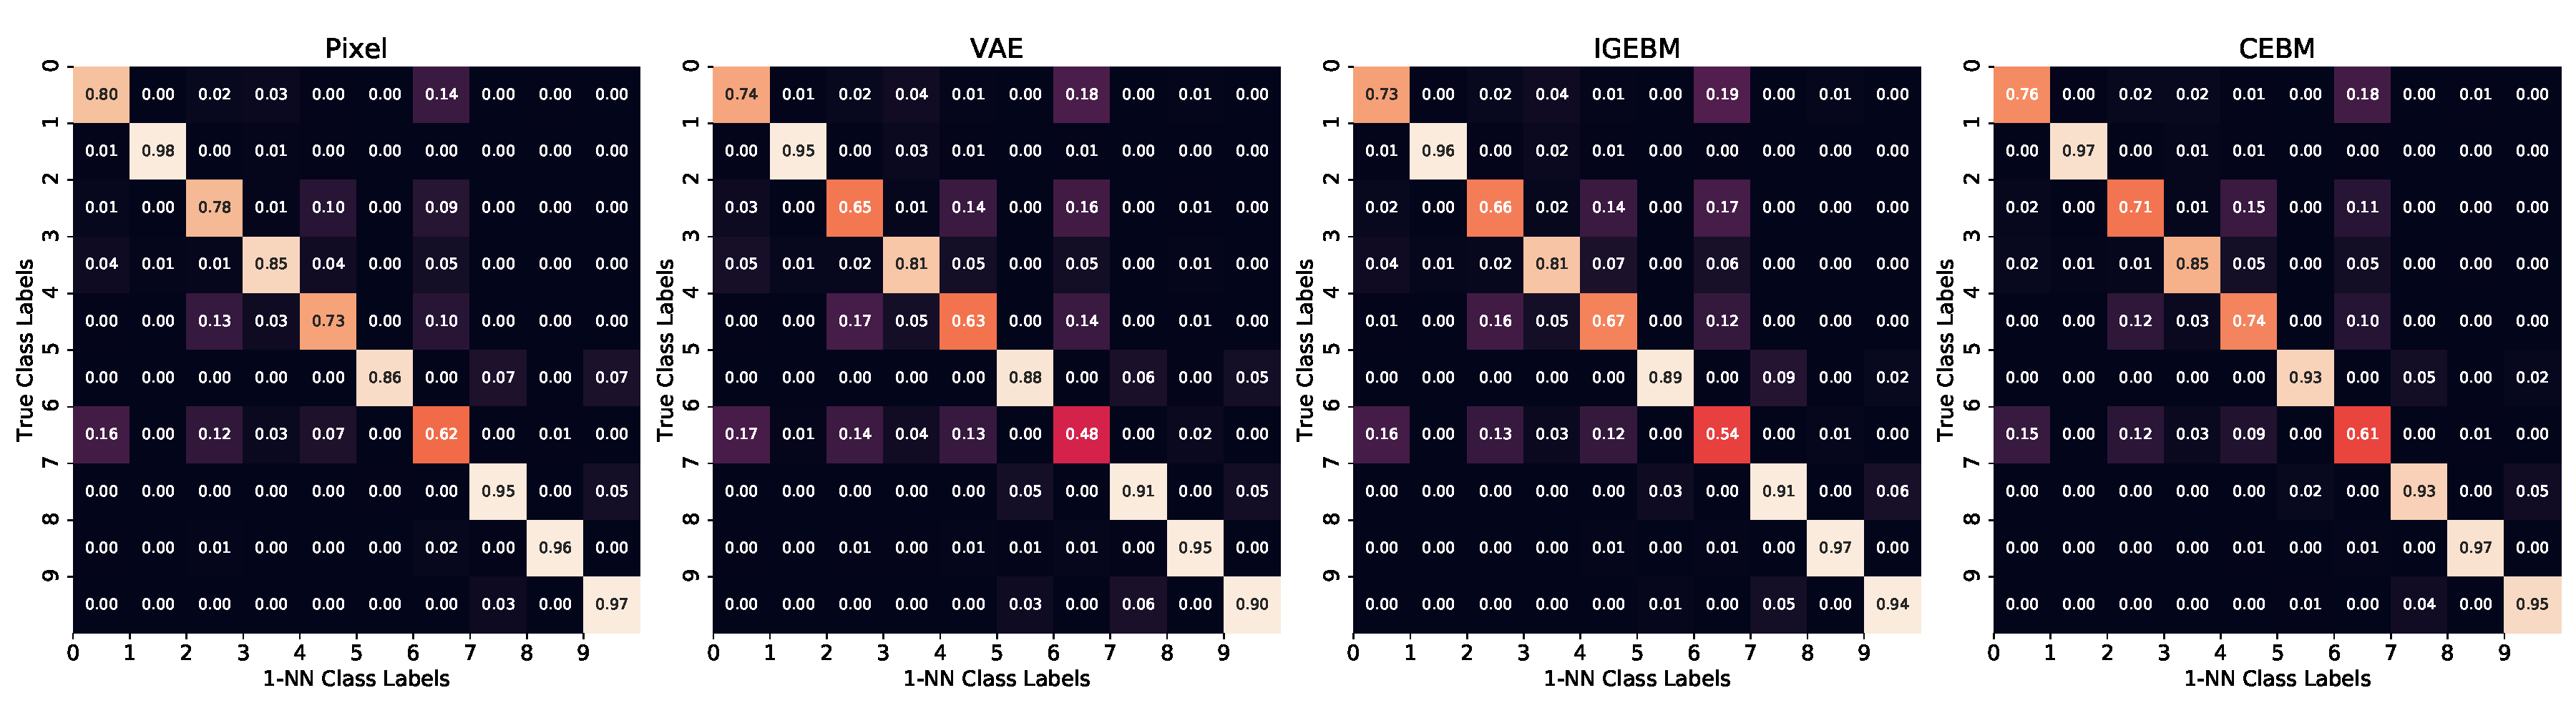
\includegraphics[width=\linewidth]{figures/confusion_matrix_14row_fashionmnist.pdf}
\caption{Fashion-MNIST}
\label{appendix:confusion-matrices-fmnist}
\end{figure}
\vspace{-2em}
\begin{figure}[!h]
\centering
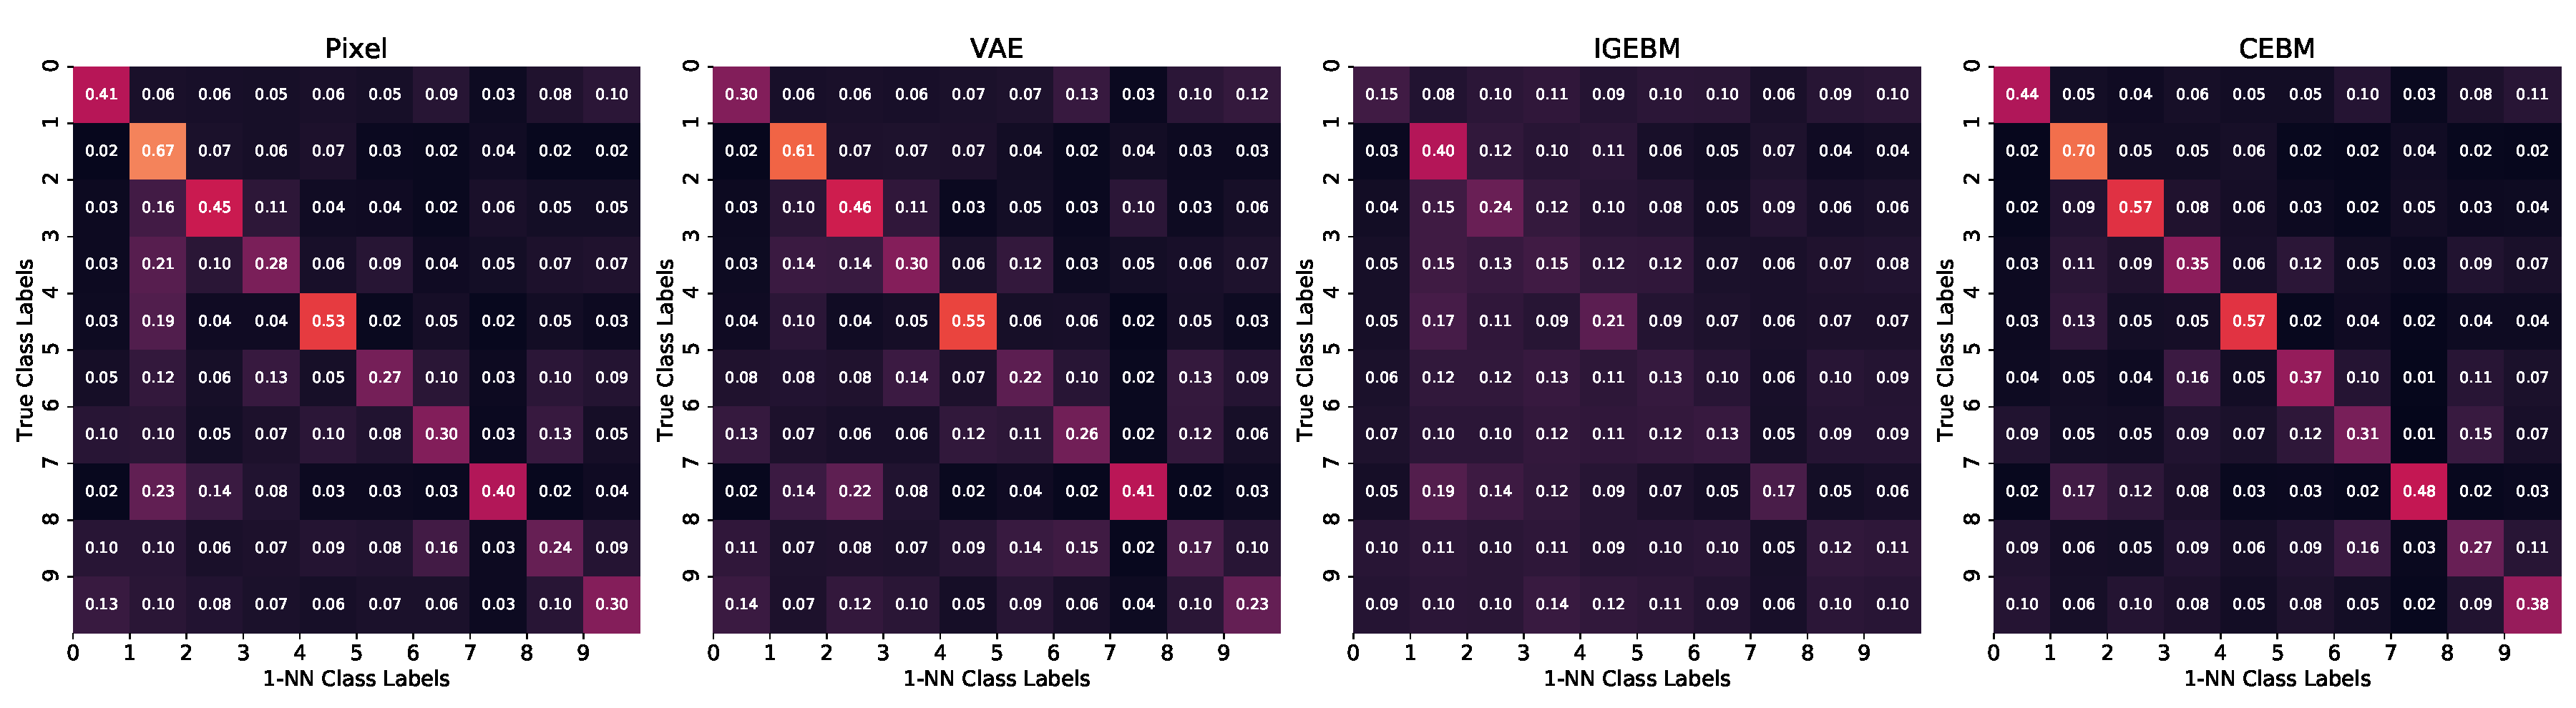
\includegraphics[width=\linewidth]{figures/confusion_matrix_14row_svhn.pdf}
\caption{SVHN}
\label{appendix:confusion-matrices-svhn}
\end{figure}
\vspace{-2em}
\begin{figure}[!h]
\centering
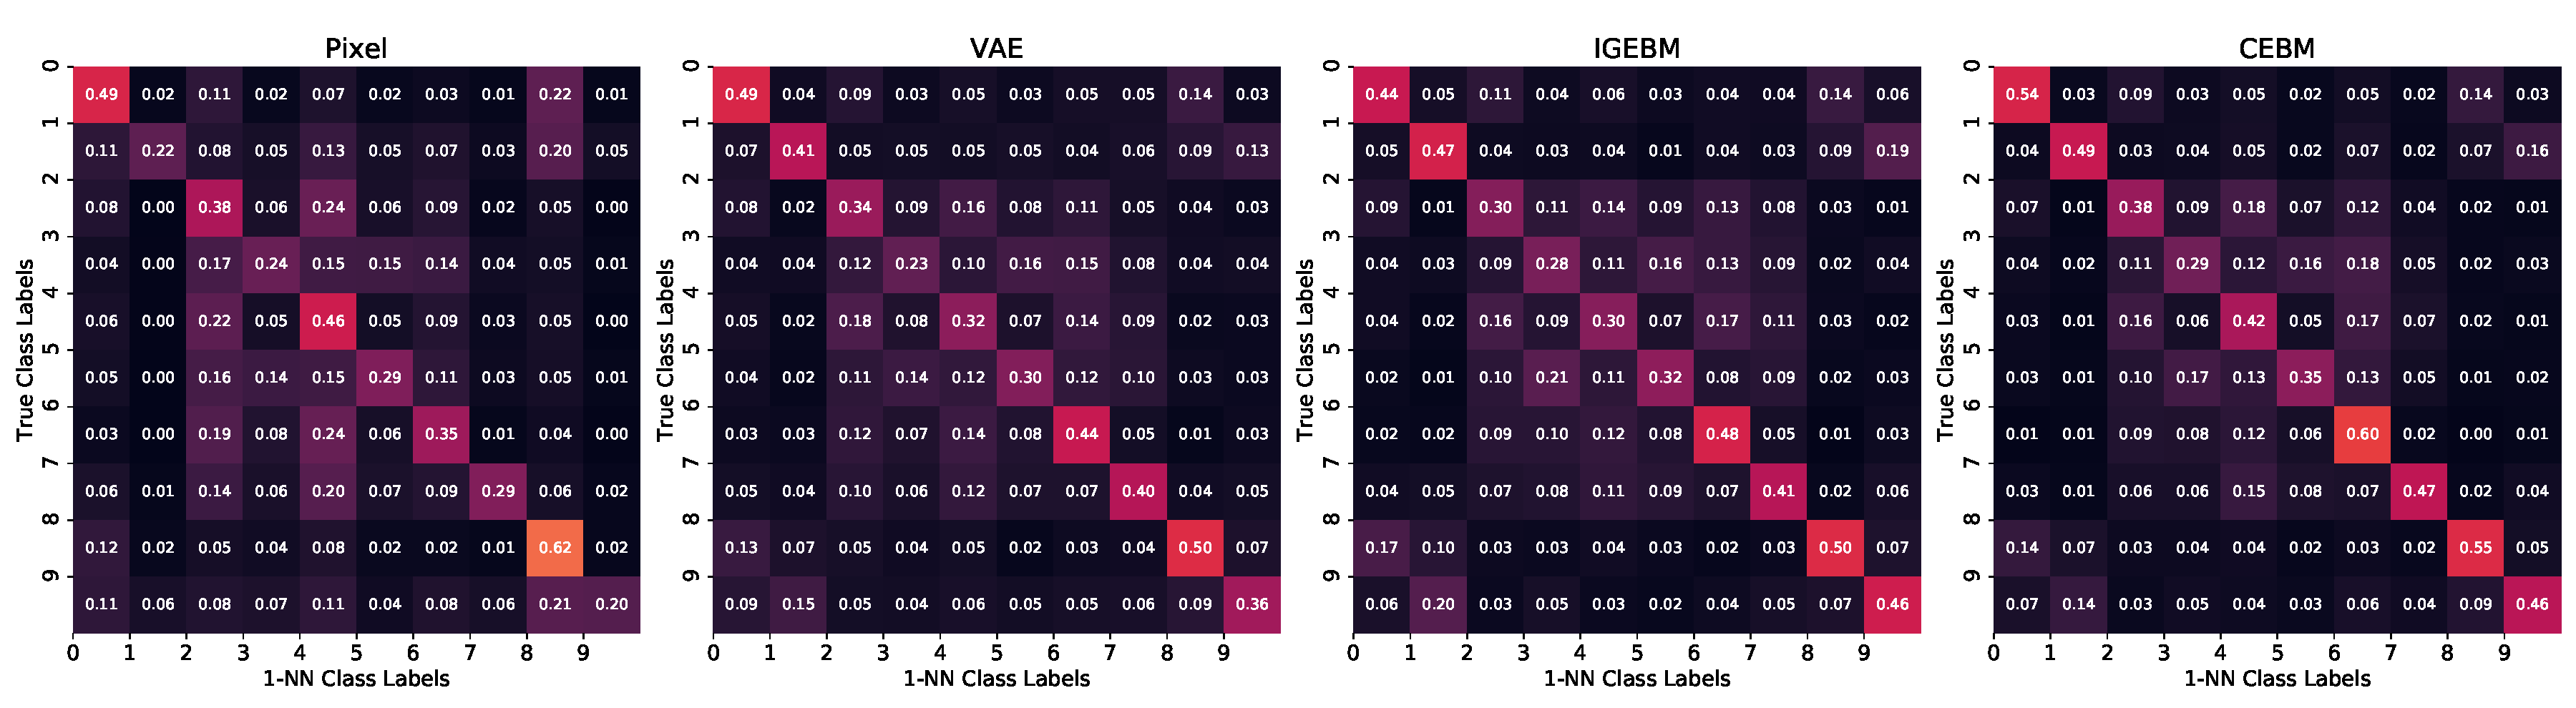
\includegraphics[width=\linewidth]{figures/confusion_matrix_14row_cifar10.pdf}
\caption{CIFAR10}
\label{appendix:confusion-matrices-cifar10}
\end{figure}

\newpage
\subsection{Out-of-Distribution Detection}
\label{appendix-sec:ood-detection}
We compute the AUROC score in OOD detection based on two different score functions.
\setlength{\tabcolsep}{4.5pt}
\begin{table*}[!h]
\caption{AUROC scores in OOD Detection. We use $\log p_{\q}(\x)$ and $\| \nabla_{\x}\log p_{\q}(\x)\|$ as score functions.The left block shows results of the models trained on F-MNIST and tested on MNIST, E-MNIST, Constant (C); The right block shows results of the models trained on CIFAR-10 and tested on SVHN, Texture and Constant (C).}
\centering
\begin{tabular}{l|ccc|ccc||ccc|ccc}
\toprule
& \multicolumn{6}{c||}{Fashion-MNIST} &    \multicolumn{6}{c}{CIFAR-10}\\
& \multicolumn{3}{c|}{$\log p_{\q}(\x)$} & \multicolumn{3}{c||}{$\| \nabla_{\x}\log p_{\q}(\x)\|$} &  \multicolumn{3}{c|}{$\log p_{\q}(\x)$} & \multicolumn{3}{c}{$\| \nabla_{\x}\log p_{\q}(\x)\|$}\\
\midrule
            &  MNIST  & E-MNIST& C &  MNIST & E-MNIST & C &  SVHN & Texture & C &  SVHN & Texture & C \\
\midrule
VAE         & .50 & .39 & .9 & .61 & .57 & .1  & .42 & \textbf{.58} & .41 & .38 & \textbf{.51} & .37 \\
IGEBM       & .35 & .36 & .90 & .78 & .82 & .96& .45 & .31 & .64 & .33 & .17 & \textbf{.62} \\
CEBM        & .37 & .34 & .90 & \textbf{.82} & \textbf{.89} & \textbf{.98} & .47 & .32 & \textbf{.66} & .31 & .17 & .54 \\
CEBMM       & \textbf{.56} & \textbf{.56} & \textbf{.92} & .56 & .80 & .95     & \textbf{.55} & .30 & .62 & \textbf{.40} & .23 & \textbf{.62}  \\
\bottomrule
\end{tabular}
\label{app:tab:ood-detection}
\end{table*}
% \end{document}

\begin{algorithm}[!t]
\caption{Persistent Contrastive Divergence}
\label{alg:cebm}
\begin{algorithmic}[1]
\State \textbf{input:} $p_\text{data}(\cdot)$, $\q$, $\alpha$, $T$
\State $\mathcal{B} \gets \{x_b \sim \mathcal{U} \text{ \textbf{for}}\ b = 1 \ldots \text{buffer-size} \}$
\While{not converged}
\State $x \sim p_\text{data}(x)$
\State $x' \sim \mathcal{B}$ with 95\% probability and $\mathcal{U}$ otherwise
\For{$t = 1 \ldots T$}
\State $\epsilon \sim \mathcal{N}(0, \alpha)$
\State $x' \gets x' - \frac{\alpha}{2} \nabla_{x} E_\q (x') + \epsilon$
\EndFor
% \State $\vx^{-} \gets \vx^{-}.\text{detach()} $
\State $\Delta_{\q} \gets \nabla_{\q} E_{\q}(x) - \nabla_{\q} E_\q(x')$  
\State $\q \gets \text{Adam}(\q, \Delta_{\q})$
\State $\mathcal{B}[x'] \gets x'$
\EndWhile
\State \textbf{return} $\q$
\end{algorithmic}
\end{algorithm}
% \section{Do \emph{not} have an appendix here}

% \textbf{\emph{Do not put content after the references.}}
% %
% Put anything that you might normally include after the references in a separate
% supplementary file.

% We recommend that you build supplementary material in a separate document.
% If you must create one PDF and cut it up, please be careful to use a tool that
% doesn't alter the margins, and that doesn't aggressively rewrite the PDF file.
% pdftk usually works fine. 

% \textbf{Please do not use Apple's preview to cut off supplementary material.} In
% previous years it has altered margins, and created headaches at the camera-ready
% stage. 
%%%%%%%%%%%%%%%%%%%%%%%%%%%%%%%%%%%%%%%%%%%%%%%%%%%%%%%%%%%%%%%%%%%%%%%%%%%%%%%
%%%%%%%%%%%%%%%%%%%%%%%%%%%%%%%%%%%%%%%%%%%%%%%%%%%%%%%%%%%%%%%%%%%%%%%%%%%%%%%


\end{document}


% This document was modified from the file originally made available by
% Pat Langley and Andrea Danyluk for ICML-2K. This version was created
% by Iain Murray in 2018, and modified by Alexandre Bouchard in
% 2019 and 2021. Previous contributors include Dan Roy, Lise Getoor and Tobias
% Scheffer, which was slightly modified from the 2010 version by
% Thorsten Joachims & Johannes Fuernkranz, slightly modified from the
% 2009 version by Kiri Wagstaff and Sam Roweis's 2008 version, which is
% slightly modified from Prasad Tadepalli's 2007 version which is a
% lightly changed version of the previous year's version by Andrew
% Moore, which was in turn edited from those of Kristian Kersting and
% Codrina Lauth. Alex Smola contributed to the algorithmic style files.
